% Options for packages loaded elsewhere
\PassOptionsToPackage{unicode}{hyperref}
\PassOptionsToPackage{hyphens}{url}
%
\documentclass[
]{article}
\usepackage{amsmath,amssymb}
\usepackage{iftex}
\ifPDFTeX
  \usepackage[T1]{fontenc}
  \usepackage[utf8]{inputenc}
  \usepackage{textcomp} % provide euro and other symbols
\else % if luatex or xetex
  \usepackage{unicode-math} % this also loads fontspec
  \defaultfontfeatures{Scale=MatchLowercase}
  \defaultfontfeatures[\rmfamily]{Ligatures=TeX,Scale=1}
\fi
\usepackage{lmodern}
\ifPDFTeX\else
  % xetex/luatex font selection
\fi
% Use upquote if available, for straight quotes in verbatim environments
\IfFileExists{upquote.sty}{\usepackage{upquote}}{}
\IfFileExists{microtype.sty}{% use microtype if available
  \usepackage[]{microtype}
  \UseMicrotypeSet[protrusion]{basicmath} % disable protrusion for tt fonts
}{}
\makeatletter
\@ifundefined{KOMAClassName}{% if non-KOMA class
  \IfFileExists{parskip.sty}{%
    \usepackage{parskip}
  }{% else
    \setlength{\parindent}{0pt}
    \setlength{\parskip}{6pt plus 2pt minus 1pt}}
}{% if KOMA class
  \KOMAoptions{parskip=half}}
\makeatother
\usepackage{xcolor}
\usepackage[margin=1in]{geometry}
\usepackage{color}
\usepackage{fancyvrb}
\newcommand{\VerbBar}{|}
\newcommand{\VERB}{\Verb[commandchars=\\\{\}]}
\DefineVerbatimEnvironment{Highlighting}{Verbatim}{commandchars=\\\{\}}
% Add ',fontsize=\small' for more characters per line
\usepackage{framed}
\definecolor{shadecolor}{RGB}{248,248,248}
\newenvironment{Shaded}{\begin{snugshade}}{\end{snugshade}}
\newcommand{\AlertTok}[1]{\textcolor[rgb]{0.94,0.16,0.16}{#1}}
\newcommand{\AnnotationTok}[1]{\textcolor[rgb]{0.56,0.35,0.01}{\textbf{\textit{#1}}}}
\newcommand{\AttributeTok}[1]{\textcolor[rgb]{0.13,0.29,0.53}{#1}}
\newcommand{\BaseNTok}[1]{\textcolor[rgb]{0.00,0.00,0.81}{#1}}
\newcommand{\BuiltInTok}[1]{#1}
\newcommand{\CharTok}[1]{\textcolor[rgb]{0.31,0.60,0.02}{#1}}
\newcommand{\CommentTok}[1]{\textcolor[rgb]{0.56,0.35,0.01}{\textit{#1}}}
\newcommand{\CommentVarTok}[1]{\textcolor[rgb]{0.56,0.35,0.01}{\textbf{\textit{#1}}}}
\newcommand{\ConstantTok}[1]{\textcolor[rgb]{0.56,0.35,0.01}{#1}}
\newcommand{\ControlFlowTok}[1]{\textcolor[rgb]{0.13,0.29,0.53}{\textbf{#1}}}
\newcommand{\DataTypeTok}[1]{\textcolor[rgb]{0.13,0.29,0.53}{#1}}
\newcommand{\DecValTok}[1]{\textcolor[rgb]{0.00,0.00,0.81}{#1}}
\newcommand{\DocumentationTok}[1]{\textcolor[rgb]{0.56,0.35,0.01}{\textbf{\textit{#1}}}}
\newcommand{\ErrorTok}[1]{\textcolor[rgb]{0.64,0.00,0.00}{\textbf{#1}}}
\newcommand{\ExtensionTok}[1]{#1}
\newcommand{\FloatTok}[1]{\textcolor[rgb]{0.00,0.00,0.81}{#1}}
\newcommand{\FunctionTok}[1]{\textcolor[rgb]{0.13,0.29,0.53}{\textbf{#1}}}
\newcommand{\ImportTok}[1]{#1}
\newcommand{\InformationTok}[1]{\textcolor[rgb]{0.56,0.35,0.01}{\textbf{\textit{#1}}}}
\newcommand{\KeywordTok}[1]{\textcolor[rgb]{0.13,0.29,0.53}{\textbf{#1}}}
\newcommand{\NormalTok}[1]{#1}
\newcommand{\OperatorTok}[1]{\textcolor[rgb]{0.81,0.36,0.00}{\textbf{#1}}}
\newcommand{\OtherTok}[1]{\textcolor[rgb]{0.56,0.35,0.01}{#1}}
\newcommand{\PreprocessorTok}[1]{\textcolor[rgb]{0.56,0.35,0.01}{\textit{#1}}}
\newcommand{\RegionMarkerTok}[1]{#1}
\newcommand{\SpecialCharTok}[1]{\textcolor[rgb]{0.81,0.36,0.00}{\textbf{#1}}}
\newcommand{\SpecialStringTok}[1]{\textcolor[rgb]{0.31,0.60,0.02}{#1}}
\newcommand{\StringTok}[1]{\textcolor[rgb]{0.31,0.60,0.02}{#1}}
\newcommand{\VariableTok}[1]{\textcolor[rgb]{0.00,0.00,0.00}{#1}}
\newcommand{\VerbatimStringTok}[1]{\textcolor[rgb]{0.31,0.60,0.02}{#1}}
\newcommand{\WarningTok}[1]{\textcolor[rgb]{0.56,0.35,0.01}{\textbf{\textit{#1}}}}
\usepackage{graphicx}
\makeatletter
\def\maxwidth{\ifdim\Gin@nat@width>\linewidth\linewidth\else\Gin@nat@width\fi}
\def\maxheight{\ifdim\Gin@nat@height>\textheight\textheight\else\Gin@nat@height\fi}
\makeatother
% Scale images if necessary, so that they will not overflow the page
% margins by default, and it is still possible to overwrite the defaults
% using explicit options in \includegraphics[width, height, ...]{}
\setkeys{Gin}{width=\maxwidth,height=\maxheight,keepaspectratio}
% Set default figure placement to htbp
\makeatletter
\def\fps@figure{htbp}
\makeatother
\setlength{\emergencystretch}{3em} % prevent overfull lines
\providecommand{\tightlist}{%
  \setlength{\itemsep}{0pt}\setlength{\parskip}{0pt}}
\setcounter{secnumdepth}{-\maxdimen} % remove section numbering
\ifLuaTeX
\usepackage[bidi=basic]{babel}
\else
\usepackage[bidi=default]{babel}
\fi
\babelprovide[main,import]{russian}
% get rid of language-specific shorthands (see #6817):
\let\LanguageShortHands\languageshorthands
\def\languageshorthands#1{}
\ifLuaTeX
  \usepackage{selnolig}  % disable illegal ligatures
\fi
\usepackage{bookmark}
\IfFileExists{xurl.sty}{\usepackage{xurl}}{} % add URL line breaks if available
\urlstyle{same}
\hypersetup{
  pdftitle={SSAMethodCode},
  pdfauthor={Yakovlev D.M.},
  pdflang={russian},
  hidelinks,
  pdfcreator={LaTeX via pandoc}}

\title{SSAMethodCode}
\author{Yakovlev D.M.}
\date{2023-06-07}

\begin{document}
\maketitle

\section{Список рукописных
функций}\label{ux441ux43fux438ux441ux43eux43a-ux440ux443ux43aux43eux43fux438ux441ux43dux44bux445-ux444ux443ux43dux43aux446ux438ux439}

\begin{Shaded}
\begin{Highlighting}[]
\CommentTok{\# Строит траекторную матрицу из временного ряда с длиной окна L}
\NormalTok{BuildTrajectoryMatrix}\OtherTok{\textless{}{-}}\ControlFlowTok{function}\NormalTok{(timeSeries, L)\{}

\NormalTok{  timeSeries }\OtherTok{\textless{}{-}} \FunctionTok{as.vector}\NormalTok{(timeSeries)}

  \CommentTok{\# Длина окна не должна превосходить длину временного ряда}
  \ControlFlowTok{if}\NormalTok{(}\FunctionTok{length}\NormalTok{(timeSeries) }\SpecialCharTok{\textless{}=}\NormalTok{ L) }\FunctionTok{stop}\NormalTok{(}\StringTok{"L parameter (window length) must be less than timeSeries length"}\NormalTok{)}


\NormalTok{  K }\OtherTok{\textless{}{-}} \FunctionTok{length}\NormalTok{(timeSeries) }\SpecialCharTok{{-}}\NormalTok{ L }\SpecialCharTok{+} \DecValTok{1}

  \CommentTok{\# Инициализация траекторной матрицы}
\NormalTok{  matrixResult }\OtherTok{\textless{}{-}} \FunctionTok{matrix}\NormalTok{(}\DecValTok{0}\NormalTok{, }\AttributeTok{ncol =}\NormalTok{ K, }\AttributeTok{nrow =}\NormalTok{ L)}

  \ControlFlowTok{for}\NormalTok{ (i }\ControlFlowTok{in} \DecValTok{1}\SpecialCharTok{:}\NormalTok{K) \{}
\NormalTok{    matrixResult[,i]}\OtherTok{\textless{}{-}}\NormalTok{timeSeries[i}\SpecialCharTok{:}\NormalTok{(i}\SpecialCharTok{+}\NormalTok{L}\DecValTok{{-}1}\NormalTok{)]}
\NormalTok{  \}}

  \FunctionTok{return}\NormalTok{(matrixResult)}
\NormalTok{\}}

\CommentTok{\# Функция диагонального усреднения}
\NormalTok{DiagonalAveraging }\OtherTok{\textless{}{-}} \ControlFlowTok{function}\NormalTok{(x)\{}
\NormalTok{  x }\OtherTok{\textless{}{-}} \FunctionTok{as.matrix}\NormalTok{(x)}

  \CommentTok{\# Если длина окна больше числа окон {-} транспонируем матрицу}
  \ControlFlowTok{if}\NormalTok{(}\FunctionTok{dim}\NormalTok{(x)[}\DecValTok{1}\NormalTok{] }\SpecialCharTok{\textgreater{}} \FunctionTok{dim}\NormalTok{(x)[}\DecValTok{2}\NormalTok{]) x }\OtherTok{\textless{}{-}} \FunctionTok{tr}\NormalTok{(x)}

\NormalTok{  L }\OtherTok{\textless{}{-}} \FunctionTok{dim}\NormalTok{(x)[}\DecValTok{1}\NormalTok{] }\CommentTok{\# Длина окна}
\NormalTok{  K }\OtherTok{\textless{}{-}} \FunctionTok{dim}\NormalTok{(x)[}\DecValTok{2}\NormalTok{] }\CommentTok{\# Число окон}
\NormalTok{  N }\OtherTok{\textless{}{-}}\NormalTok{ L }\SpecialCharTok{+}\NormalTok{ K }\SpecialCharTok{{-}} \DecValTok{1} \CommentTok{\# Длина ряда}

  \FunctionTok{print}\NormalTok{(}\FunctionTok{paste}\NormalTok{(}\StringTok{"L = "}\NormalTok{, L, }\StringTok{"K = "}\NormalTok{, K, }\StringTok{"N = "}\NormalTok{, N))}


\NormalTok{  timeSeriesResult }\OtherTok{\textless{}{-}} \FunctionTok{c}\NormalTok{()}

  \CommentTok{\# Восстановление компоненты ряда (по формуле с тремя случаями)}

  \CommentTok{\# Случай один}
  \ControlFlowTok{for}\NormalTok{(i }\ControlFlowTok{in} \DecValTok{1}\SpecialCharTok{:}\NormalTok{L)\{}
\NormalTok{    temporaryValue }\OtherTok{\textless{}{-}} \DecValTok{0}

    \ControlFlowTok{for}\NormalTok{(j }\ControlFlowTok{in} \DecValTok{1}\SpecialCharTok{:}\NormalTok{i)\{}
\NormalTok{      temporaryValue }\OtherTok{=}\NormalTok{ temporaryValue }\SpecialCharTok{+}\NormalTok{ x[j, i }\SpecialCharTok{{-}}\NormalTok{ j }\SpecialCharTok{+} \DecValTok{1}\NormalTok{]}
\NormalTok{    \}}

\NormalTok{    timeSeriesResult[i] }\OtherTok{\textless{}{-}}\NormalTok{ temporaryValue}\SpecialCharTok{/}\NormalTok{i}
\NormalTok{  \}}

  \CommentTok{\# Случай два}
  \ControlFlowTok{for}\NormalTok{(i }\ControlFlowTok{in}\NormalTok{ (L}\SpecialCharTok{+}\DecValTok{1}\NormalTok{)}\SpecialCharTok{:}\NormalTok{K)\{}
\NormalTok{    temporaryValue }\OtherTok{\textless{}{-}} \DecValTok{0}

    \ControlFlowTok{for}\NormalTok{(j }\ControlFlowTok{in} \DecValTok{1}\SpecialCharTok{:}\NormalTok{L)\{}
\NormalTok{      temporaryValue }\OtherTok{=}\NormalTok{ temporaryValue }\SpecialCharTok{+}\NormalTok{ x[j, i }\SpecialCharTok{{-}}\NormalTok{ j }\SpecialCharTok{+} \DecValTok{1}\NormalTok{]}
\NormalTok{    \}}

\NormalTok{    timeSeriesResult[i] }\OtherTok{\textless{}{-}}\NormalTok{ temporaryValue}\SpecialCharTok{/}\NormalTok{L}
\NormalTok{  \}}

  \CommentTok{\# Случай три}
  \ControlFlowTok{for}\NormalTok{(i }\ControlFlowTok{in}\NormalTok{ (K}\SpecialCharTok{+}\DecValTok{1}\NormalTok{)}\SpecialCharTok{:}\NormalTok{N)\{}
\NormalTok{    temporaryValue }\OtherTok{\textless{}{-}} \DecValTok{0}

    \ControlFlowTok{for}\NormalTok{(j }\ControlFlowTok{in}\NormalTok{ (i }\SpecialCharTok{{-}}\NormalTok{ K }\SpecialCharTok{+} \DecValTok{1}\NormalTok{)}\SpecialCharTok{:}\NormalTok{L)\{}
\NormalTok{      temporaryValue }\OtherTok{=}\NormalTok{ temporaryValue }\SpecialCharTok{+}\NormalTok{ x[j, i }\SpecialCharTok{{-}}\NormalTok{ j }\SpecialCharTok{+} \DecValTok{1}\NormalTok{]}
\NormalTok{    \}}

\NormalTok{    timeSeriesResult[i] }\OtherTok{\textless{}{-}}\NormalTok{ temporaryValue}\SpecialCharTok{/}\NormalTok{(N}\SpecialCharTok{{-}}\NormalTok{i}\SpecialCharTok{+}\DecValTok{1}\NormalTok{)}
\NormalTok{  \}}

  \FunctionTok{return}\NormalTok{(timeSeriesResult)}
\NormalTok{\}}

\CommentTok{\# Функция, возвращающая конечный ранг ряда в случае его существования}
\NormalTok{TimeSeriesFiniteRank }\OtherTok{\textless{}{-}} \ControlFlowTok{function}\NormalTok{(timeSeries)\{}
  
\NormalTok{  N }\OtherTok{\textless{}{-}} \FunctionTok{length}\NormalTok{(timeSeries)     }\CommentTok{\# Длина ряда}
  
\NormalTok{  rnkCurr }\OtherTok{\textless{}{-}} \DecValTok{0}                \CommentTok{\# Ранг}
\NormalTok{  rnkList }\OtherTok{\textless{}{-}} \FunctionTok{c}\NormalTok{()}
  
\NormalTok{  upperBound }\OtherTok{\textless{}{-}}\NormalTok{ (N }\SpecialCharTok{+}\NormalTok{ N}\SpecialCharTok{\%\%}\DecValTok{2}\NormalTok{)}\SpecialCharTok{/}\DecValTok{2}  \CommentTok{\# Верхняя граница проверки (до половины длины ряда)}
  
  \ControlFlowTok{for}\NormalTok{(L }\ControlFlowTok{in} \DecValTok{2}\SpecialCharTok{:}\NormalTok{upperBound)\{}
\NormalTok{    rnkStep }\OtherTok{\textless{}{-}} \FunctionTok{qr}\NormalTok{(}\FunctionTok{BuildTrajectoryMatrix}\NormalTok{(timeSeries, L))}\SpecialCharTok{$}\NormalTok{rank }
    
\NormalTok{    rnkList }\OtherTok{=} \FunctionTok{c}\NormalTok{(rnkList, rnkStep)}
    
    \ControlFlowTok{if}\NormalTok{(rnkStep }\SpecialCharTok{\textgreater{}=}\NormalTok{ rnkCurr) rnkCurr }\OtherTok{\textless{}{-}}\NormalTok{ rnkStep}
    \ControlFlowTok{else}\NormalTok{ \{}
      \FunctionTok{print}\NormalTok{(}\StringTok{"Found a bad rank sequence: "}\NormalTok{)}
      \FunctionTok{return}\NormalTok{(}\DecValTok{0}\NormalTok{)}
\NormalTok{    \}}
\NormalTok{  \}}
  
  \FunctionTok{print}\NormalTok{(rnkList)}
  
  \FunctionTok{return}\NormalTok{(rnkCurr)}
\NormalTok{\}}


\CommentTok{\# Создание экспоненциально{-}модулированного гармонического ряда}
\NormalTok{CreateExponentialTimeSeries }\OtherTok{\textless{}{-}} \ControlFlowTok{function}\NormalTok{(A, alpha, freq, angle, N)\{}
\NormalTok{  timeSeries }\OtherTok{\textless{}{-}} \FunctionTok{c}\NormalTok{()}
  
  \CommentTok{\# Проверка на плохие случаи (частота, угол, длина ряда вне диапазона)}
  \ControlFlowTok{if}\NormalTok{(N }\SpecialCharTok{\textless{}=} \DecValTok{0}\NormalTok{) }\FunctionTok{stop}\NormalTok{(}\StringTok{"Error: N \textless{}= 0"}\NormalTok{)}
  \ControlFlowTok{if}\NormalTok{( freq }\SpecialCharTok{\textgreater{}}\NormalTok{ (}\DecValTok{1}\SpecialCharTok{/}\DecValTok{2}\NormalTok{) }\SpecialCharTok{||}\NormalTok{ freq }\SpecialCharTok{\textless{}} \DecValTok{0}\NormalTok{) }\FunctionTok{stop}\NormalTok{(}\StringTok{"Error: frequency is out of bounds"}\NormalTok{)}
  \ControlFlowTok{if}\NormalTok{(angle }\SpecialCharTok{\textgreater{}=} \DecValTok{2}\SpecialCharTok{*}\NormalTok{pi }\SpecialCharTok{||}\NormalTok{ angle }\SpecialCharTok{\textless{}} \DecValTok{0}\NormalTok{) }\FunctionTok{stop}\NormalTok{(}\StringTok{"Error: angle is out of bounds"}\NormalTok{)}
  
  \CommentTok{\# Построение временного ряда}
  \ControlFlowTok{for}\NormalTok{(n }\ControlFlowTok{in} \DecValTok{0}\SpecialCharTok{:}\NormalTok{(N}\DecValTok{{-}1}\NormalTok{))\{}
\NormalTok{    timeSeries }\OtherTok{\textless{}{-}} \FunctionTok{c}\NormalTok{(timeSeries, A}\SpecialCharTok{*}\FunctionTok{exp}\NormalTok{(alpha}\SpecialCharTok{*}\NormalTok{n)}\SpecialCharTok{*}\FunctionTok{cos}\NormalTok{(}\DecValTok{2}\SpecialCharTok{*}\NormalTok{pi}\SpecialCharTok{*}\NormalTok{freq}\SpecialCharTok{*}\NormalTok{n }\SpecialCharTok{+}\NormalTok{ angle))}
\NormalTok{  \}}
  
  \FunctionTok{return}\NormalTok{(timeSeries)}
\NormalTok{\}}


\CommentTok{\# Создание полиномиального ряда}
\NormalTok{CreatePolynomialTimeSeries }\OtherTok{\textless{}{-}} \ControlFlowTok{function}\NormalTok{(coefficientVector, N)\{}
\NormalTok{  timeSeries }\OtherTok{\textless{}{-}} \FunctionTok{c}\NormalTok{()}
  
  \CommentTok{\# Проверка на корректность ввода вектора коэффициентов полинома}
  \ControlFlowTok{if}\NormalTok{(}\FunctionTok{typeof}\NormalTok{(coefficientVector) }\SpecialCharTok{!=} \StringTok{"double"} \SpecialCharTok{\&\&} \FunctionTok{typeof}\NormalTok{(coefficientVector) }\SpecialCharTok{!=} \StringTok{"vector"}\NormalTok{) }\FunctionTok{stop}\NormalTok{(}\StringTok{"Error: wrong coefficient type"}\NormalTok{)}
  
  \CommentTok{\# Построение временного ряда}
  \ControlFlowTok{for}\NormalTok{(i }\ControlFlowTok{in} \DecValTok{0}\SpecialCharTok{:}\NormalTok{(N}\DecValTok{{-}1}\NormalTok{))\{}
\NormalTok{    x }\OtherTok{\textless{}{-}} \DecValTok{0}
    
    \ControlFlowTok{for}\NormalTok{(j }\ControlFlowTok{in} \DecValTok{1}\SpecialCharTok{:}\FunctionTok{length}\NormalTok{(coefficientVector))\{}
\NormalTok{      x }\OtherTok{=}\NormalTok{ x }\SpecialCharTok{+}\NormalTok{ coefficientVector[j]}\SpecialCharTok{*}\NormalTok{i}\SpecialCharTok{\^{}}\NormalTok{(j}\DecValTok{{-}1}\NormalTok{)}
\NormalTok{    \}}
    
\NormalTok{    timeSeries }\OtherTok{\textless{}{-}} \FunctionTok{c}\NormalTok{(timeSeries, x)}
\NormalTok{  \}}
  
  \FunctionTok{return}\NormalTok{(timeSeries)}
\NormalTok{\}}


\CommentTok{\# Создание полиномиального ряда с отрицательными степенями}
\NormalTok{CreateReversePolynomialTimeSeries }\OtherTok{\textless{}{-}} \ControlFlowTok{function}\NormalTok{(coefficientVector, N)\{}
\NormalTok{  timeSeries }\OtherTok{\textless{}{-}} \FunctionTok{c}\NormalTok{()}
  
  \CommentTok{\# Проверка на корректность ввода вектора коэффициентов полинома}
  \ControlFlowTok{if}\NormalTok{(}\FunctionTok{typeof}\NormalTok{(coefficientVector) }\SpecialCharTok{!=} \StringTok{"double"} \SpecialCharTok{\&\&} \FunctionTok{typeof}\NormalTok{(coefficientVector) }\SpecialCharTok{!=} \StringTok{"vector"}\NormalTok{) }\FunctionTok{stop}\NormalTok{(}\StringTok{"Error: wrong coefficient type"}\NormalTok{)}
  
  \CommentTok{\# Построение временного ряда}
\NormalTok{  timeSeries }\OtherTok{\textless{}{-}} \FunctionTok{c}\NormalTok{(timeSeries, coefficientVector[}\DecValTok{1}\NormalTok{])}
  
  \ControlFlowTok{for}\NormalTok{(i }\ControlFlowTok{in} \DecValTok{1}\SpecialCharTok{:}\NormalTok{(N}\DecValTok{{-}1}\NormalTok{))\{}
\NormalTok{    x }\OtherTok{\textless{}{-}} \DecValTok{0}
    
    \ControlFlowTok{for}\NormalTok{(j }\ControlFlowTok{in} \DecValTok{1}\SpecialCharTok{:}\FunctionTok{length}\NormalTok{(coefficientVector))\{}
\NormalTok{      x }\OtherTok{=}\NormalTok{ x }\SpecialCharTok{+}\NormalTok{ coefficientVector[j]}\SpecialCharTok{*}\NormalTok{i}\SpecialCharTok{\^{}}\NormalTok{(}\DecValTok{1}\SpecialCharTok{{-}}\NormalTok{j)}
\NormalTok{    \}}
    
\NormalTok{    timeSeries }\OtherTok{\textless{}{-}} \FunctionTok{c}\NormalTok{(timeSeries, x)}
\NormalTok{  \}}
  
  \FunctionTok{return}\NormalTok{(timeSeries)}
\NormalTok{\}}

\CommentTok{\# Создание временного ряда от степенного ряда}
\NormalTok{CreatePowerTimeSeries }\OtherTok{\textless{}{-}} \ControlFlowTok{function}\NormalTok{(coefficientVector, x, x0, N, }\AttributeTok{Reverse =} \ConstantTok{FALSE}\NormalTok{)\{}
\NormalTok{  timeSeries }\OtherTok{\textless{}{-}} \FunctionTok{c}\NormalTok{()}
  
  \CommentTok{\# Проверка на корректность ввода вектора коэффициентов полинома}
  \ControlFlowTok{if}\NormalTok{(}\FunctionTok{typeof}\NormalTok{(coefficientVector) }\SpecialCharTok{!=} \StringTok{"double"} \SpecialCharTok{\&\&} \FunctionTok{typeof}\NormalTok{(coefficientVector) }\SpecialCharTok{!=} \StringTok{"vector"}\NormalTok{) }\FunctionTok{stop}\NormalTok{(}\StringTok{"Error: wrong coefficient type"}\NormalTok{)}
  
  \CommentTok{\# Построение временного ряда}
  \ControlFlowTok{if}\NormalTok{(Reverse)\{}
    \ControlFlowTok{for}\NormalTok{(i }\ControlFlowTok{in} \DecValTok{0}\SpecialCharTok{:}\NormalTok{(N}\DecValTok{{-}1}\NormalTok{))\{}
\NormalTok{      xResult }\OtherTok{\textless{}{-}}\NormalTok{ coefficientVector[i]}\SpecialCharTok{*}\NormalTok{(x}\SpecialCharTok{{-}}\NormalTok{x0)}\SpecialCharTok{\^{}}\NormalTok{(}\SpecialCharTok{{-}}\NormalTok{i)}
    
\NormalTok{      timeSeries }\OtherTok{\textless{}{-}} \FunctionTok{c}\NormalTok{(timeSeries, xResult)  }
\NormalTok{    \}}
\NormalTok{  \}}
  \ControlFlowTok{else}\NormalTok{\{}
    \ControlFlowTok{for}\NormalTok{(i }\ControlFlowTok{in} \DecValTok{0}\SpecialCharTok{:}\NormalTok{(N}\DecValTok{{-}1}\NormalTok{))\{}
\NormalTok{      xResult }\OtherTok{\textless{}{-}}\NormalTok{ coefficientVector[i]}\SpecialCharTok{*}\NormalTok{(x }\SpecialCharTok{{-}}\NormalTok{ x0)}\SpecialCharTok{\^{}}\NormalTok{i}
      
\NormalTok{      timeSeries }\OtherTok{\textless{}{-}} \FunctionTok{c}\NormalTok{(timeSeries, xResult)}
\NormalTok{    \}}
\NormalTok{  \}}
  \FunctionTok{return}\NormalTok{(timeSeries)}
\NormalTok{\}}



\CommentTok{\# Создание логарифмического ряда}
\NormalTok{CreateLogarithmicTimeSeries }\OtherTok{\textless{}{-}} \ControlFlowTok{function}\NormalTok{(A, }\AttributeTok{logBase =} \FunctionTok{exp}\NormalTok{(}\DecValTok{1}\NormalTok{), coefficientVector, N)\{}
\NormalTok{  timeSeries }\OtherTok{\textless{}{-}} \FunctionTok{c}\NormalTok{()}
  
  
  \CommentTok{\# Проверка на корректность ввода вектора коэффициентов полинома}
  \ControlFlowTok{if}\NormalTok{(}\FunctionTok{typeof}\NormalTok{(coefficientVector) }\SpecialCharTok{!=} \StringTok{"double"} \SpecialCharTok{\&\&} \FunctionTok{typeof}\NormalTok{(coefficientVector) }\SpecialCharTok{!=} \StringTok{"vector"}\NormalTok{) }\FunctionTok{stop}\NormalTok{(}\StringTok{"Error: wrong coefficient type"}\NormalTok{)}
  
  \CommentTok{\# Построение временного ряда}
  \ControlFlowTok{for}\NormalTok{(i }\ControlFlowTok{in} \DecValTok{0}\SpecialCharTok{:}\NormalTok{(N}\DecValTok{{-}1}\NormalTok{))\{}
\NormalTok{    x }\OtherTok{\textless{}{-}} \DecValTok{0}
    
    \ControlFlowTok{for}\NormalTok{(j }\ControlFlowTok{in} \DecValTok{1}\SpecialCharTok{:}\FunctionTok{length}\NormalTok{(coefficientVector))\{}
\NormalTok{      x }\OtherTok{=}\NormalTok{ x }\SpecialCharTok{+}\NormalTok{ coefficientVector[j]}\SpecialCharTok{*}\NormalTok{i}\SpecialCharTok{\^{}}\NormalTok{(j}\DecValTok{{-}1}\NormalTok{)}
\NormalTok{    \}}
    
\NormalTok{    x }\OtherTok{=}\NormalTok{ A}\SpecialCharTok{*}\FunctionTok{log}\NormalTok{(x, logBase)}
    
\NormalTok{    timeSeries }\OtherTok{\textless{}{-}} \FunctionTok{c}\NormalTok{(timeSeries, x)}
\NormalTok{  \}}
  
  \FunctionTok{return}\NormalTok{(timeSeries)}
\NormalTok{\}}
\end{Highlighting}
\end{Shaded}

\section{Графические изображения исследуемых временных
рядов}\label{ux433ux440ux430ux444ux438ux447ux435ux441ux43aux438ux435-ux438ux437ux43eux431ux440ux430ux436ux435ux43dux438ux44f-ux438ux441ux441ux43bux435ux434ux443ux435ux43cux44bux445-ux432ux440ux435ux43cux435ux43dux43dux44bux445-ux440ux44fux434ux43eux432}

\begin{Shaded}
\begin{Highlighting}[]
\FunctionTok{library}\NormalTok{(Rssa)}
\end{Highlighting}
\end{Shaded}

\begin{verbatim}
## Загрузка требуемого пакета: svd
\end{verbatim}

\begin{verbatim}
## Загрузка требуемого пакета: forecast
\end{verbatim}

\begin{verbatim}
## Registered S3 method overwritten by 'quantmod':
##   method            from
##   as.zoo.data.frame zoo
\end{verbatim}

\begin{verbatim}
## 
## Присоединяю пакет: 'Rssa'
\end{verbatim}

\begin{verbatim}
## Следующий объект скрыт от 'package:stats':
## 
##     decompose
\end{verbatim}

\begin{Shaded}
\begin{Highlighting}[]
\NormalTok{timeSeries}\OtherTok{\textless{}{-}}\FunctionTok{CreateExponentialTimeSeries}\NormalTok{(}\DecValTok{2}\NormalTok{, }\FloatTok{1e{-}4}\NormalTok{, }\DecValTok{1}\SpecialCharTok{/}\DecValTok{5}\NormalTok{, pi, }\DecValTok{100}\NormalTok{)}

\NormalTok{test}\OtherTok{\textless{}{-}}\FunctionTok{ssa}\NormalTok{(timeSeries)}

\NormalTok{timeSeries}
\end{Highlighting}
\end{Shaded}

\begin{verbatim}
##   [1] -2.0000000 -0.6180958  1.6183576  1.6185195 -0.6182813 -2.0010003
##   [7] -0.6184049  1.6191670  1.6193289 -0.6185905 -2.0020010 -0.6187142
##  [13]  1.6199768  1.6201388 -0.6188998 -2.0030023 -0.6190236  1.6207870
##  [19]  1.6209491 -0.6192094 -2.0040040 -0.6193332  1.6215976  1.6217597
##  [25] -0.6195191 -2.0050063 -0.6196430  1.6224086  1.6225708 -0.6198289
##  [31] -2.0060090 -0.6199529  1.6232200  1.6233823 -0.6201389 -2.0070123
##  [37] -0.6202629  1.6240318  1.6241942 -0.6204490 -2.0080160 -0.6205731
##  [43]  1.6248440  1.6250065 -0.6207593 -2.0090203 -0.6208835  1.6256566
##  [49]  1.6258192 -0.6210698 -2.0100250 -0.6211940  1.6264697  1.6266323
##  [55] -0.6213804 -2.0110303 -0.6215047  1.6272831  1.6274459 -0.6216912
##  [61] -2.0120361 -0.6218155  1.6280970  1.6282598 -0.6220021 -2.0130423
##  [67] -0.6221265  1.6289112  1.6290741 -0.6223132 -2.0140491 -0.6224376
##  [73]  1.6297259  1.6298889 -0.6226244 -2.0150564 -0.6227489  1.6305409
##  [79]  1.6307040 -0.6229358 -2.0160642 -0.6230604  1.6313564  1.6315196
##  [85] -0.6232473 -2.0170725 -0.6233720  1.6321723  1.6323355 -0.6235590
##  [91] -2.0180812 -0.6236838  1.6329886  1.6331519 -0.6238709 -2.0190905
##  [97] -0.6239957  1.6338053  1.6339687 -0.6241829
\end{verbatim}

\begin{Shaded}
\begin{Highlighting}[]
\FunctionTok{set.seed}\NormalTok{(}\DecValTok{2023}\NormalTok{)}
\end{Highlighting}
\end{Shaded}

\section{Задача 1.}\label{ux437ux430ux434ux430ux447ux430-1.}

Наблюдение 1. Поскольку каждый вид временного ряда, рассматриваемый при
построении другого ряда, имеет свой базис (пусть их ранги будут r1, r2,
\ldots, rk; N - длина ряда), то их линейная комбинация будет

\begin{enumerate}
\def\labelenumi{\arabic{enumi}.}
\tightlist
\item
  Рядом конечного ранга R
\item
  R = min\{r1+r2+\ldots+rk, N \%/\% 2 + N\%\%2\}
\end{enumerate}

\subsection{Пример 1. Сильная и слабая
разделимости}\label{ux43fux440ux438ux43cux435ux440-1.-ux441ux438ux43bux44cux43dux430ux44f-ux438-ux441ux43bux430ux431ux430ux44f-ux440ux430ux437ux434ux435ux43bux438ux43cux43eux441ux442ux438}

\begin{Shaded}
\begin{Highlighting}[]
\CommentTok{\# Созданные ряды удовлетворяют условию слабой разделимости (см.}
\CommentTok{\# предложение 2.1., стр. 14), однако разделимость может быть как сильной,}
\CommentTok{\# так и слабой, в зависимости от параметра.}

\CommentTok{\# Рассмотрим периодический и константный ряды. Для них существуют}
\CommentTok{\# параметры функций и параметры метода L и K = N {-} L + 1, при которых они}
\CommentTok{\# разделимы.}

\CommentTok{\# Возьмём периодический ряд со значением элемента }
\CommentTok{\# f\_n = 2*cos(pi*n/2) 0 \textless{}= n\textless{}= 6 }

\NormalTok{PeriodicTS }\OtherTok{\textless{}{-}} \FunctionTok{CreateExponentialTimeSeries}\NormalTok{(}\DecValTok{2}\NormalTok{, }\DecValTok{0}\NormalTok{, }\DecValTok{1}\SpecialCharTok{/}\DecValTok{4}\NormalTok{, }\DecValTok{0}\NormalTok{, }\DecValTok{7}\NormalTok{)}

\CommentTok{\# При SVD получим сингулярное число кратности два со значением 4.}
\FunctionTok{svd}\NormalTok{(}\FunctionTok{BuildTrajectoryMatrix}\NormalTok{(PeriodicTS, }\DecValTok{4}\NormalTok{))}
\end{Highlighting}
\end{Shaded}

\begin{verbatim}
## $d
## [1] 4.000000e+00 4.000000e+00 2.627267e-16 2.795263e-32
## 
## $u
##               [,1]          [,2]      [,3]       [,4]
## [1,] -7.071068e-01 -4.395601e-17 0.4225771 -0.5669467
## [2,] -4.329637e-17  7.071068e-01 0.5669467  0.4225771
## [3,]  7.071068e-01  1.292295e-16 0.4225771 -0.5669467
## [4,]  1.298891e-16 -7.071068e-01 0.5669467  0.4225771
## 
## $v
##               [,1]          [,2]         [,3]          [,4]
## [1,] -7.071068e-01  6.162976e-33 1.570092e-16 -7.071068e-01
## [2,]  0.000000e+00 -7.071068e-01 7.071068e-01  1.110223e-16
## [3,]  7.071068e-01 -1.110223e-16 0.000000e+00 -7.071068e-01
## [4,]  8.659275e-17  7.071068e-01 7.071068e-01  7.041650e-17
\end{verbatim}

\begin{Shaded}
\begin{Highlighting}[]
\CommentTok{\# Возьмём константный ряд со значением ряда f\_n = 1, 0 \textbackslash{}leq n \textbackslash{}leq 6}
\NormalTok{ConstTS }\OtherTok{\textless{}{-}} \FunctionTok{rep}\NormalTok{(}\DecValTok{1}\NormalTok{, }\DecValTok{7}\NormalTok{)}

\CommentTok{\# При SVD получим сингулярное число со значением 4.}
\FunctionTok{svd}\NormalTok{(}\FunctionTok{BuildTrajectoryMatrix}\NormalTok{(ConstTS, }\DecValTok{4}\NormalTok{)) }
\end{Highlighting}
\end{Shaded}

\begin{verbatim}
## $d
## [1] 4.000000e+00 3.330669e-16 0.000000e+00 0.000000e+00
## 
## $u
##      [,1]       [,2]       [,3]          [,4]
## [1,] -0.5  0.8660254  0.0000000 -4.163336e-17
## [2,] -0.5 -0.2886751 -0.5773503 -5.773503e-01
## [3,] -0.5 -0.2886751 -0.2113249  7.886751e-01
## [4,] -0.5 -0.2886751  0.7886751 -2.113249e-01
## 
## $v
##      [,1]       [,2]       [,3]       [,4]
## [1,] -0.5  0.8660254  0.0000000  0.0000000
## [2,] -0.5 -0.2886751 -0.5773503 -0.5773503
## [3,] -0.5 -0.2886751 -0.2113249  0.7886751
## [4,] -0.5 -0.2886751  0.7886751 -0.2113249
\end{verbatim}

\begin{Shaded}
\begin{Highlighting}[]
\CommentTok{\#Построив временный ряд из их суммы}

\NormalTok{TSWOutNoise }\OtherTok{\textless{}{-}}\NormalTok{ PeriodicTS }\SpecialCharTok{+}\NormalTok{ ConstTS }
\NormalTok{SSAWOutNoise }\OtherTok{\textless{}{-}} \FunctionTok{ssa}\NormalTok{(TSWOutNoise) }
\CommentTok{\# В ходе SVD получилось три сингулярных числа со значением 4, которые нельзя}
\CommentTok{\# однозначно разделить между собой}

\NormalTok{m }\OtherTok{\textless{}{-}} \FunctionTok{svd}\NormalTok{(}\FunctionTok{BuildTrajectoryMatrix}\NormalTok{(TSWOutNoise, }\DecValTok{4}\NormalTok{))}
\FunctionTok{TimeSeriesFiniteRank}\NormalTok{(TSWOutNoise)}
\end{Highlighting}
\end{Shaded}

\begin{verbatim}
## [1] 2 3 3
\end{verbatim}

\begin{verbatim}
## [1] 3
\end{verbatim}

\begin{Shaded}
\begin{Highlighting}[]
\FunctionTok{plot}\NormalTok{(SSAWOutNoise, }\AttributeTok{idx=}\DecValTok{1}\SpecialCharTok{:}\DecValTok{3}\NormalTok{)}
\end{Highlighting}
\end{Shaded}

\includegraphics{SSAMethodCode_files/figure-latex/unnamed-chunk-2-1.pdf}

\begin{Shaded}
\begin{Highlighting}[]
\FunctionTok{plot}\NormalTok{(SSAWOutNoise, }\AttributeTok{type=}\StringTok{\textquotesingle{}vectors\textquotesingle{}}\NormalTok{, }\AttributeTok{idx=}\DecValTok{1}\SpecialCharTok{:}\DecValTok{3}\NormalTok{)}
\end{Highlighting}
\end{Shaded}

\includegraphics{SSAMethodCode_files/figure-latex/unnamed-chunk-2-2.pdf}

\begin{Shaded}
\begin{Highlighting}[]
\FunctionTok{plot}\NormalTok{(SSAWOutNoise, }\AttributeTok{type=}\StringTok{\textquotesingle{}vectors\textquotesingle{}}\NormalTok{, }\AttributeTok{vectors=}\StringTok{\textquotesingle{}factor\textquotesingle{}}\NormalTok{, }\AttributeTok{idx=}\DecValTok{1}\SpecialCharTok{:}\DecValTok{3}\NormalTok{)}
\end{Highlighting}
\end{Shaded}

\includegraphics{SSAMethodCode_files/figure-latex/unnamed-chunk-2-3.pdf}

\begin{Shaded}
\begin{Highlighting}[]
\FunctionTok{plot}\NormalTok{(SSAWOutNoise, }\AttributeTok{type=}\StringTok{\textquotesingle{}series\textquotesingle{}}\NormalTok{, }\AttributeTok{groups=}\DecValTok{1}\SpecialCharTok{:}\DecValTok{3}\NormalTok{)}
\end{Highlighting}
\end{Shaded}

\includegraphics{SSAMethodCode_files/figure-latex/unnamed-chunk-2-4.pdf}

\begin{Shaded}
\begin{Highlighting}[]
\FunctionTok{plot}\NormalTok{(SSAWOutNoise, }\AttributeTok{type=}\StringTok{\textquotesingle{}paired\textquotesingle{}}\NormalTok{, }\AttributeTok{idx=}\DecValTok{1}\SpecialCharTok{:}\DecValTok{2}\NormalTok{)}
\end{Highlighting}
\end{Shaded}

\includegraphics{SSAMethodCode_files/figure-latex/unnamed-chunk-2-5.pdf}

\begin{Shaded}
\begin{Highlighting}[]
\FunctionTok{plot}\NormalTok{(}\FunctionTok{wcor}\NormalTok{(SSAWOutNoise, }\AttributeTok{groups=}\DecValTok{1}\SpecialCharTok{:}\DecValTok{3}\NormalTok{), }\AttributeTok{scales=}\FunctionTok{list}\NormalTok{(}\FunctionTok{c}\NormalTok{(}\DecValTok{1}\NormalTok{,}\DecValTok{2}\NormalTok{,}\DecValTok{3}\NormalTok{)))}
\end{Highlighting}
\end{Shaded}

\includegraphics{SSAMethodCode_files/figure-latex/unnamed-chunk-2-6.pdf}

Графически, в случае слабой разделимости, вместо константного ряда
получается ряд, напоминающий периодический, из-за чего разделить и
определить компоненты ряда становится невозможным.

Если же, например, изменить коэффициент в периодическом ряде, то все
компоненты можно легко разделить.

\begin{Shaded}
\begin{Highlighting}[]
\NormalTok{PeriodicTS\_New }\OtherTok{\textless{}{-}} \FunctionTok{CreateExponentialTimeSeries}\NormalTok{(}\DecValTok{3}\NormalTok{, }\DecValTok{0}\NormalTok{, }\DecValTok{1}\SpecialCharTok{/}\DecValTok{4}\NormalTok{, }\DecValTok{0}\NormalTok{, }\DecValTok{7}\NormalTok{)}
\NormalTok{TSAWOutNoise\_New }\OtherTok{\textless{}{-}}\NormalTok{ PeriodicTS\_New }\SpecialCharTok{+}\NormalTok{ ConstTS}
\NormalTok{SSAWOutNoise\_New }\OtherTok{\textless{}{-}} \FunctionTok{ssa}\NormalTok{(TSAWOutNoise\_New)}

\FunctionTok{plot}\NormalTok{(SSAWOutNoise\_New)}
\end{Highlighting}
\end{Shaded}

\includegraphics{SSAMethodCode_files/figure-latex/unnamed-chunk-3-1.pdf}

\begin{Shaded}
\begin{Highlighting}[]
\FunctionTok{plot}\NormalTok{(SSAWOutNoise\_New, }\AttributeTok{type=}\StringTok{\textquotesingle{}vectors\textquotesingle{}}\NormalTok{, }\AttributeTok{idx=}\DecValTok{1}\SpecialCharTok{:}\DecValTok{3}\NormalTok{)}
\end{Highlighting}
\end{Shaded}

\includegraphics{SSAMethodCode_files/figure-latex/unnamed-chunk-3-2.pdf}

\begin{Shaded}
\begin{Highlighting}[]
\FunctionTok{plot}\NormalTok{(SSAWOutNoise\_New, }\AttributeTok{type=}\StringTok{\textquotesingle{}vectors\textquotesingle{}}\NormalTok{, }\AttributeTok{vectors=}\StringTok{\textquotesingle{}factor\textquotesingle{}}\NormalTok{, }\AttributeTok{idx=}\DecValTok{1}\SpecialCharTok{:}\DecValTok{3}\NormalTok{)}
\end{Highlighting}
\end{Shaded}

\includegraphics{SSAMethodCode_files/figure-latex/unnamed-chunk-3-3.pdf}

\begin{Shaded}
\begin{Highlighting}[]
\FunctionTok{plot}\NormalTok{(SSAWOutNoise\_New, }\AttributeTok{type=}\StringTok{\textquotesingle{}series\textquotesingle{}}\NormalTok{, }\AttributeTok{groups=}\DecValTok{1}\SpecialCharTok{:}\DecValTok{3}\NormalTok{)}
\end{Highlighting}
\end{Shaded}

\includegraphics{SSAMethodCode_files/figure-latex/unnamed-chunk-3-4.pdf}

\begin{Shaded}
\begin{Highlighting}[]
\FunctionTok{plot}\NormalTok{(SSAWOutNoise\_New, }\AttributeTok{type=}\StringTok{\textquotesingle{}paired\textquotesingle{}}\NormalTok{, }\AttributeTok{idx=}\DecValTok{1}\SpecialCharTok{:}\DecValTok{2}\NormalTok{)}
\end{Highlighting}
\end{Shaded}

\includegraphics{SSAMethodCode_files/figure-latex/unnamed-chunk-3-5.pdf}

\begin{Shaded}
\begin{Highlighting}[]
\FunctionTok{plot}\NormalTok{(}\FunctionTok{wcor}\NormalTok{(SSAWOutNoise\_New, }\AttributeTok{groups=}\DecValTok{1}\SpecialCharTok{:}\DecValTok{3}\NormalTok{), }\AttributeTok{scales=}\FunctionTok{list}\NormalTok{(}\FunctionTok{c}\NormalTok{(}\DecValTok{1}\NormalTok{,}\DecValTok{2}\NormalTok{,}\DecValTok{3}\NormalTok{)))}
\end{Highlighting}
\end{Shaded}

\includegraphics{SSAMethodCode_files/figure-latex/unnamed-chunk-3-6.pdf}

При добавление белого шума значения сингулярных чисел не совпадают друг
с другом. Можно заметить возможность выделения тренда (константного
ряда), периодики (ряда с косинусом) и шума (с самым низким сингулярным
числом)

Однако, в случае

\begin{Shaded}
\begin{Highlighting}[]
\NormalTok{samplenorm }\OtherTok{\textless{}{-}} \FunctionTok{c}\NormalTok{(}\SpecialCharTok{{-}}\FloatTok{0.2058265}\NormalTok{, }\SpecialCharTok{{-}}\FloatTok{0.1471636}\NormalTok{, }\FloatTok{0.6092870}\NormalTok{, }\FloatTok{0.1220557}\NormalTok{, }\SpecialCharTok{{-}}\FloatTok{0.2225760}\NormalTok{, }\SpecialCharTok{{-}}\FloatTok{0.9239018}\NormalTok{, }\SpecialCharTok{{-}}\FloatTok{0.3144127}\NormalTok{)}
\end{Highlighting}
\end{Shaded}

\begin{Shaded}
\begin{Highlighting}[]
\NormalTok{TSWNoise }\OtherTok{\textless{}{-}}\NormalTok{ TSWOutNoise }\SpecialCharTok{+}\NormalTok{ samplenorm}
\NormalTok{SSAWNoise }\OtherTok{\textless{}{-}} \FunctionTok{ssa}\NormalTok{(TSWNoise) }
\FunctionTok{TimeSeriesFiniteRank}\NormalTok{(TSWNoise)}
\end{Highlighting}
\end{Shaded}

\begin{verbatim}
## [1] 2 3 4
\end{verbatim}

\begin{verbatim}
## [1] 4
\end{verbatim}

\begin{Shaded}
\begin{Highlighting}[]
\FunctionTok{plot}\NormalTok{(SSAWNoise)}
\end{Highlighting}
\end{Shaded}

\includegraphics{SSAMethodCode_files/figure-latex/unnamed-chunk-5-1.pdf}

\begin{Shaded}
\begin{Highlighting}[]
\FunctionTok{plot}\NormalTok{(SSAWNoise, }\AttributeTok{type=}\StringTok{\textquotesingle{}vectors\textquotesingle{}}\NormalTok{, }\AttributeTok{idx=}\DecValTok{1}\SpecialCharTok{:}\DecValTok{4}\NormalTok{)}
\end{Highlighting}
\end{Shaded}

\includegraphics{SSAMethodCode_files/figure-latex/unnamed-chunk-5-2.pdf}

\begin{Shaded}
\begin{Highlighting}[]
\FunctionTok{plot}\NormalTok{(SSAWNoise, }\AttributeTok{type=}\StringTok{\textquotesingle{}vectors\textquotesingle{}}\NormalTok{, }\AttributeTok{vectors=}\StringTok{\textquotesingle{}factor\textquotesingle{}}\NormalTok{, }\AttributeTok{idx=}\DecValTok{1}\SpecialCharTok{:}\DecValTok{4}\NormalTok{)}
\end{Highlighting}
\end{Shaded}

\includegraphics{SSAMethodCode_files/figure-latex/unnamed-chunk-5-3.pdf}

\begin{Shaded}
\begin{Highlighting}[]
\FunctionTok{plot}\NormalTok{(SSAWNoise, }\AttributeTok{type=}\StringTok{\textquotesingle{}series\textquotesingle{}}\NormalTok{, }\AttributeTok{groups=}\DecValTok{1}\SpecialCharTok{:}\DecValTok{4}\NormalTok{)}
\end{Highlighting}
\end{Shaded}

\includegraphics{SSAMethodCode_files/figure-latex/unnamed-chunk-5-4.pdf}

\begin{Shaded}
\begin{Highlighting}[]
\FunctionTok{plot}\NormalTok{(}\FunctionTok{wcor}\NormalTok{(SSAWNoise, }\AttributeTok{groups=}\DecValTok{1}\SpecialCharTok{:}\DecValTok{4}\NormalTok{), }\AttributeTok{scales=}\FunctionTok{list}\NormalTok{(}\FunctionTok{c}\NormalTok{(}\DecValTok{1}\NormalTok{,}\DecValTok{2}\NormalTok{,}\DecValTok{3}\NormalTok{,}\DecValTok{4}\NormalTok{)))}
\end{Highlighting}
\end{Shaded}

\includegraphics{SSAMethodCode_files/figure-latex/unnamed-chunk-5-5.pdf}

Продемонстрируем, что с ростом N точность выделения компонент ряда
возрастает.

\begin{Shaded}
\begin{Highlighting}[]
\NormalTok{PeriodicTS\_Special }\OtherTok{\textless{}{-}} \FunctionTok{CreateExponentialTimeSeries}\NormalTok{(}\DecValTok{3}\NormalTok{,}\DecValTok{0}\NormalTok{,}\DecValTok{1}\SpecialCharTok{/}\DecValTok{4}\NormalTok{,}\DecValTok{0}\NormalTok{,}\DecValTok{1000}\NormalTok{)}
\NormalTok{ConstTS\_Special }\OtherTok{\textless{}{-}} \FunctionTok{rep}\NormalTok{(}\DecValTok{1}\NormalTok{, }\DecValTok{1000}\NormalTok{)}
\NormalTok{samplenorm1000 }\OtherTok{\textless{}{-}} \FunctionTok{rnorm}\NormalTok{(}\DecValTok{1000}\NormalTok{)}
\NormalTok{samplenorm1000[}\DecValTok{1}\SpecialCharTok{:}\DecValTok{7}\NormalTok{] }\OtherTok{\textless{}{-}} \FunctionTok{c}\NormalTok{(}\SpecialCharTok{{-}}\FloatTok{0.2058265}\NormalTok{, }\SpecialCharTok{{-}}\FloatTok{0.1471636}\NormalTok{, }\FloatTok{0.6092870}\NormalTok{, }\FloatTok{0.1220557}\NormalTok{, }\SpecialCharTok{{-}}\FloatTok{0.2225760}\NormalTok{, }\SpecialCharTok{{-}}\FloatTok{0.9239018}\NormalTok{, }\SpecialCharTok{{-}}\FloatTok{0.3144127}\NormalTok{)}
\end{Highlighting}
\end{Shaded}

\begin{Shaded}
\begin{Highlighting}[]
\NormalTok{TSExample }\OtherTok{\textless{}{-}}\NormalTok{ PeriodicTS\_Special}\SpecialCharTok{+}\NormalTok{ConstTS\_Special}\SpecialCharTok{+}\NormalTok{samplenorm1000}
\CommentTok{\# TimeSeriesFiniteRank(TSExample)}
\NormalTok{s.TSExample }\OtherTok{\textless{}{-}} \FunctionTok{ssa}\NormalTok{(TSExample[}\DecValTok{1}\SpecialCharTok{:}\DecValTok{400}\NormalTok{])}
\NormalTok{r.TSExample }\OtherTok{\textless{}{-}} \FunctionTok{reconstruct}\NormalTok{(s.TSExample)}
\FunctionTok{plot}\NormalTok{(s.TSExample, }\AttributeTok{type=}\StringTok{\textquotesingle{}vectors\textquotesingle{}}\NormalTok{, }\AttributeTok{idx=}\DecValTok{1}\SpecialCharTok{:}\DecValTok{3}\NormalTok{)}
\end{Highlighting}
\end{Shaded}

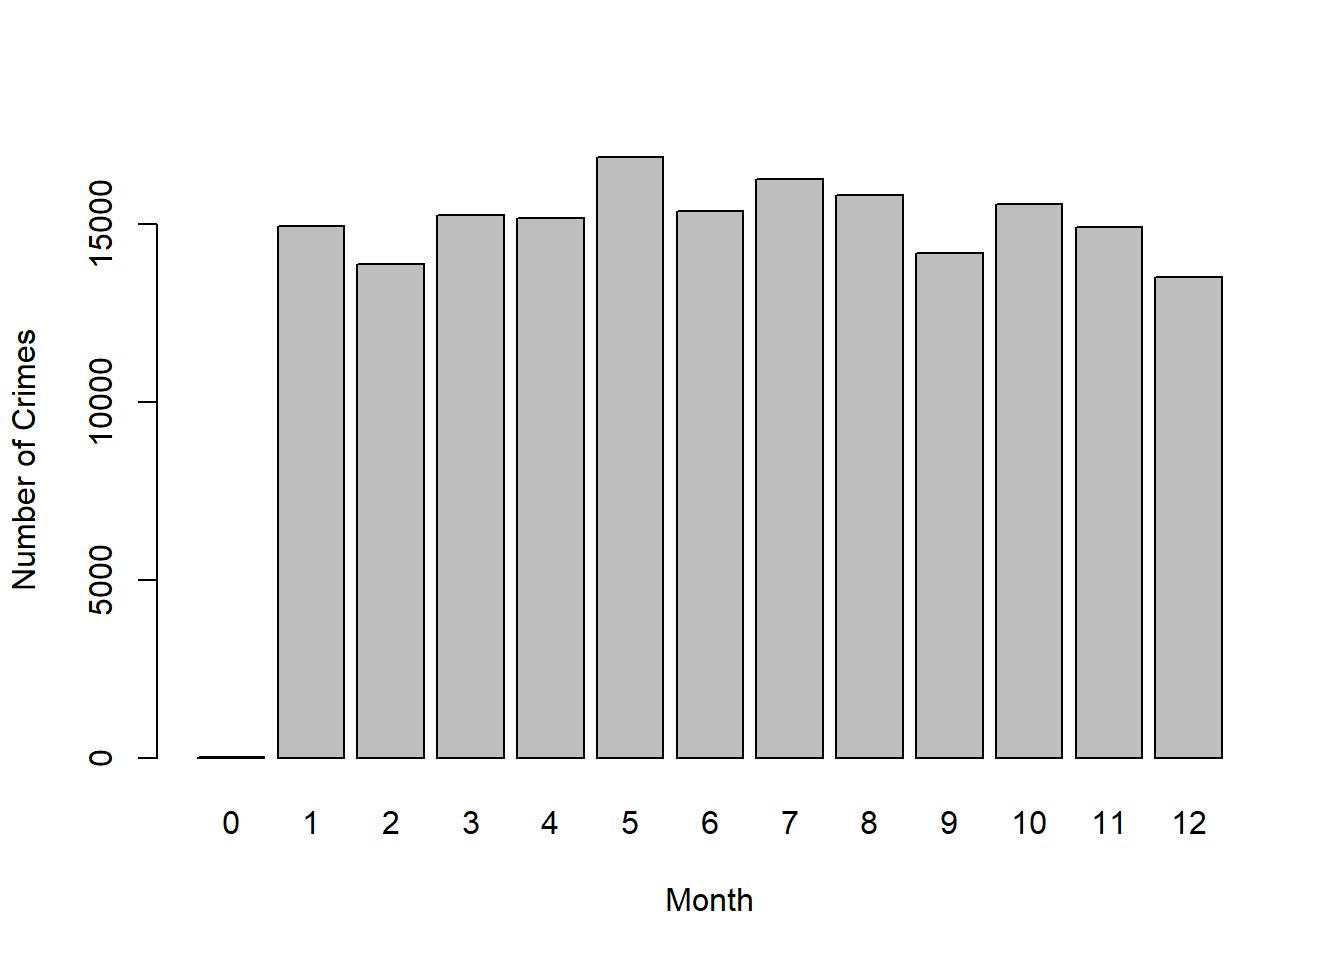
\includegraphics{SSAMethodCode_files/figure-latex/unnamed-chunk-7-1.pdf}

\begin{Shaded}
\begin{Highlighting}[]
\FunctionTok{plot}\NormalTok{(s.TSExample, }\AttributeTok{type=}\StringTok{\textquotesingle{}vectors\textquotesingle{}}\NormalTok{, }\AttributeTok{vectors=}\StringTok{\textquotesingle{}factor\textquotesingle{}}\NormalTok{, }\AttributeTok{idx=}\DecValTok{1}\SpecialCharTok{:}\DecValTok{3}\NormalTok{)}
\end{Highlighting}
\end{Shaded}

\includegraphics{SSAMethodCode_files/figure-latex/unnamed-chunk-7-2.pdf}

\begin{Shaded}
\begin{Highlighting}[]
\FunctionTok{plot}\NormalTok{(s.TSExample, }\AttributeTok{type=}\StringTok{\textquotesingle{}paired\textquotesingle{}}\NormalTok{, }\AttributeTok{idx=}\DecValTok{1}\SpecialCharTok{:}\DecValTok{2}\NormalTok{, }\AttributeTok{plot.contrib =} \ConstantTok{FALSE}\NormalTok{)}
\end{Highlighting}
\end{Shaded}

\includegraphics{SSAMethodCode_files/figure-latex/unnamed-chunk-7-3.pdf}

\begin{Shaded}
\begin{Highlighting}[]
\FunctionTok{plot}\NormalTok{(s.TSExample, }\AttributeTok{type=}\StringTok{\textquotesingle{}series\textquotesingle{}}\NormalTok{, }\AttributeTok{groups=}\DecValTok{1}\SpecialCharTok{:}\DecValTok{3}\NormalTok{)}
\end{Highlighting}
\end{Shaded}

\includegraphics{SSAMethodCode_files/figure-latex/unnamed-chunk-7-4.pdf}

\begin{Shaded}
\begin{Highlighting}[]
\FunctionTok{plot}\NormalTok{(}\FunctionTok{wcor}\NormalTok{(s.TSExample, }\AttributeTok{groups=}\DecValTok{1}\SpecialCharTok{:}\DecValTok{50}\NormalTok{), }\AttributeTok{scales=}\FunctionTok{list}\NormalTok{(}\AttributeTok{at=}\FunctionTok{seq}\NormalTok{(}\DecValTok{5}\NormalTok{, }\DecValTok{50}\NormalTok{, }\DecValTok{5}\NormalTok{)))}
\end{Highlighting}
\end{Shaded}

\includegraphics{SSAMethodCode_files/figure-latex/unnamed-chunk-7-5.pdf}

\begin{Shaded}
\begin{Highlighting}[]
\FunctionTok{plot}\NormalTok{(r.TSExample)}
\end{Highlighting}
\end{Shaded}

\includegraphics{SSAMethodCode_files/figure-latex/unnamed-chunk-7-6.pdf}

\begin{Shaded}
\begin{Highlighting}[]
\NormalTok{s.TSExample }\OtherTok{\textless{}{-}} \FunctionTok{ssa}\NormalTok{(TSExample[}\DecValTok{1}\SpecialCharTok{:}\DecValTok{200}\NormalTok{])}
\NormalTok{r.TSExample }\OtherTok{\textless{}{-}} \FunctionTok{reconstruct}\NormalTok{(s.TSExample)}
\FunctionTok{plot}\NormalTok{(s.TSExample, }\AttributeTok{type=}\StringTok{\textquotesingle{}vectors\textquotesingle{}}\NormalTok{, }\AttributeTok{idx=}\DecValTok{1}\SpecialCharTok{:}\DecValTok{3}\NormalTok{)}
\end{Highlighting}
\end{Shaded}

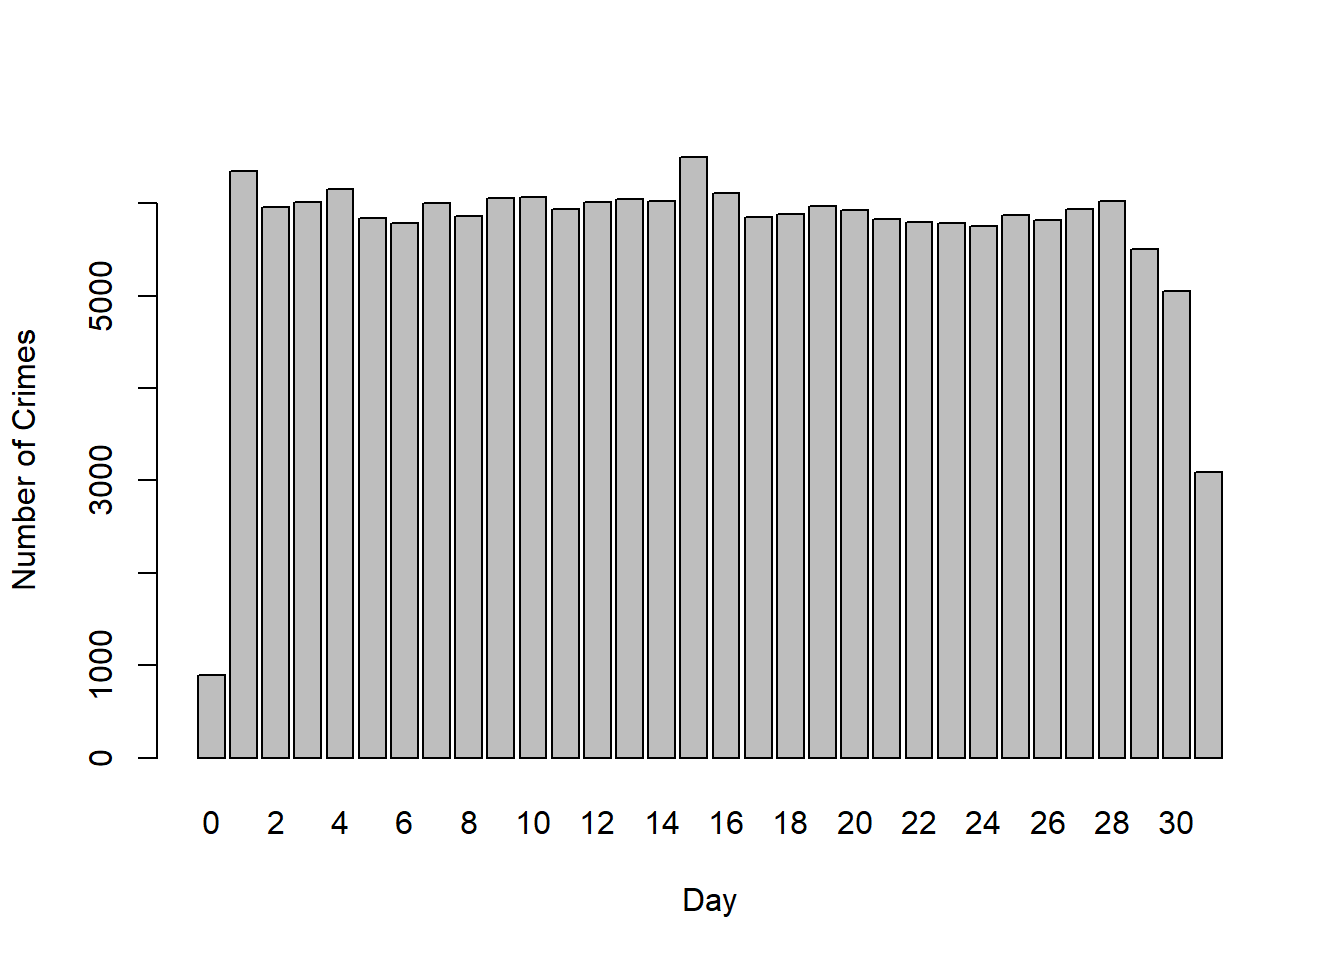
\includegraphics{SSAMethodCode_files/figure-latex/unnamed-chunk-8-1.pdf}

\begin{Shaded}
\begin{Highlighting}[]
\FunctionTok{plot}\NormalTok{(s.TSExample, }\AttributeTok{type=}\StringTok{\textquotesingle{}vectors\textquotesingle{}}\NormalTok{, }\AttributeTok{vectors=}\StringTok{\textquotesingle{}factor\textquotesingle{}}\NormalTok{, }\AttributeTok{idx=}\DecValTok{1}\SpecialCharTok{:}\DecValTok{3}\NormalTok{)}
\end{Highlighting}
\end{Shaded}

\includegraphics{SSAMethodCode_files/figure-latex/unnamed-chunk-8-2.pdf}

\begin{Shaded}
\begin{Highlighting}[]
\FunctionTok{plot}\NormalTok{(s.TSExample, }\AttributeTok{type=}\StringTok{\textquotesingle{}paired\textquotesingle{}}\NormalTok{, }\AttributeTok{idx=}\DecValTok{1}\SpecialCharTok{:}\DecValTok{2}\NormalTok{, }\AttributeTok{plot.contrib =} \ConstantTok{FALSE}\NormalTok{)}
\end{Highlighting}
\end{Shaded}

\includegraphics{SSAMethodCode_files/figure-latex/unnamed-chunk-8-3.pdf}

\begin{Shaded}
\begin{Highlighting}[]
\FunctionTok{plot}\NormalTok{(s.TSExample, }\AttributeTok{type=}\StringTok{\textquotesingle{}series\textquotesingle{}}\NormalTok{, }\AttributeTok{groups=}\DecValTok{1}\SpecialCharTok{:}\DecValTok{3}\NormalTok{)}
\end{Highlighting}
\end{Shaded}

\includegraphics{SSAMethodCode_files/figure-latex/unnamed-chunk-8-4.pdf}

\begin{Shaded}
\begin{Highlighting}[]
\FunctionTok{plot}\NormalTok{(}\FunctionTok{wcor}\NormalTok{(s.TSExample, }\AttributeTok{groups=}\DecValTok{1}\SpecialCharTok{:}\DecValTok{50}\NormalTok{), }\AttributeTok{scales=}\FunctionTok{list}\NormalTok{(}\AttributeTok{at=}\FunctionTok{seq}\NormalTok{(}\DecValTok{5}\NormalTok{,}\DecValTok{50}\NormalTok{,}\DecValTok{5}\NormalTok{)))}
\end{Highlighting}
\end{Shaded}

\includegraphics{SSAMethodCode_files/figure-latex/unnamed-chunk-8-5.pdf}

\begin{Shaded}
\begin{Highlighting}[]
\FunctionTok{plot}\NormalTok{(r.TSExample)}
\end{Highlighting}
\end{Shaded}

\includegraphics{SSAMethodCode_files/figure-latex/unnamed-chunk-8-6.pdf}

\begin{Shaded}
\begin{Highlighting}[]
\NormalTok{s.TSExample }\OtherTok{\textless{}{-}} \FunctionTok{ssa}\NormalTok{(TSExample[}\DecValTok{1}\SpecialCharTok{:}\DecValTok{100}\NormalTok{])}
\NormalTok{r.TSExample }\OtherTok{\textless{}{-}} \FunctionTok{reconstruct}\NormalTok{(s.TSExample)}
\FunctionTok{plot}\NormalTok{(s.TSExample, }\AttributeTok{type=}\StringTok{\textquotesingle{}vectors\textquotesingle{}}\NormalTok{, }\AttributeTok{idx=}\DecValTok{1}\SpecialCharTok{:}\DecValTok{3}\NormalTok{)}
\end{Highlighting}
\end{Shaded}

\includegraphics{SSAMethodCode_files/figure-latex/unnamed-chunk-9-1.pdf}

\begin{Shaded}
\begin{Highlighting}[]
\FunctionTok{plot}\NormalTok{(s.TSExample, }\AttributeTok{type=}\StringTok{\textquotesingle{}vectors\textquotesingle{}}\NormalTok{, }\AttributeTok{vectors=}\StringTok{\textquotesingle{}factor\textquotesingle{}}\NormalTok{, }\AttributeTok{idx=}\DecValTok{1}\SpecialCharTok{:}\DecValTok{3}\NormalTok{)}
\end{Highlighting}
\end{Shaded}

\includegraphics{SSAMethodCode_files/figure-latex/unnamed-chunk-9-2.pdf}

\begin{Shaded}
\begin{Highlighting}[]
\FunctionTok{plot}\NormalTok{(s.TSExample, }\AttributeTok{type=}\StringTok{\textquotesingle{}paired\textquotesingle{}}\NormalTok{, }\AttributeTok{idx=}\DecValTok{1}\SpecialCharTok{:}\DecValTok{2}\NormalTok{, }\AttributeTok{plot.contrib =} \ConstantTok{FALSE}\NormalTok{)}
\end{Highlighting}
\end{Shaded}

\includegraphics{SSAMethodCode_files/figure-latex/unnamed-chunk-9-3.pdf}

\begin{Shaded}
\begin{Highlighting}[]
\FunctionTok{plot}\NormalTok{(s.TSExample, }\AttributeTok{type=}\StringTok{\textquotesingle{}series\textquotesingle{}}\NormalTok{, }\AttributeTok{groups=}\DecValTok{1}\SpecialCharTok{:}\DecValTok{3}\NormalTok{)}
\end{Highlighting}
\end{Shaded}

\includegraphics{SSAMethodCode_files/figure-latex/unnamed-chunk-9-4.pdf}

\begin{Shaded}
\begin{Highlighting}[]
\FunctionTok{plot}\NormalTok{(}\FunctionTok{wcor}\NormalTok{(s.TSExample, }\AttributeTok{groups=}\DecValTok{1}\SpecialCharTok{:}\DecValTok{25}\NormalTok{), }\AttributeTok{scales=}\FunctionTok{list}\NormalTok{(}\AttributeTok{at=}\FunctionTok{seq}\NormalTok{(}\DecValTok{5}\NormalTok{,}\DecValTok{25}\NormalTok{,}\DecValTok{5}\NormalTok{)))}
\end{Highlighting}
\end{Shaded}

\includegraphics{SSAMethodCode_files/figure-latex/unnamed-chunk-9-5.pdf}

\begin{Shaded}
\begin{Highlighting}[]
\FunctionTok{plot}\NormalTok{(r.TSExample)}
\end{Highlighting}
\end{Shaded}

\includegraphics{SSAMethodCode_files/figure-latex/unnamed-chunk-9-6.pdf}

\begin{Shaded}
\begin{Highlighting}[]
\NormalTok{s.TSExample }\OtherTok{\textless{}{-}} \FunctionTok{ssa}\NormalTok{(TSExample[}\DecValTok{1}\SpecialCharTok{:}\DecValTok{50}\NormalTok{])}
\NormalTok{r.TSExample }\OtherTok{\textless{}{-}} \FunctionTok{reconstruct}\NormalTok{(s.TSExample)}
\FunctionTok{plot}\NormalTok{(s.TSExample, }\AttributeTok{type=}\StringTok{\textquotesingle{}vectors\textquotesingle{}}\NormalTok{, }\AttributeTok{idx=}\DecValTok{1}\SpecialCharTok{:}\DecValTok{3}\NormalTok{)}
\end{Highlighting}
\end{Shaded}

\includegraphics{SSAMethodCode_files/figure-latex/unnamed-chunk-10-1.pdf}

\begin{Shaded}
\begin{Highlighting}[]
\FunctionTok{plot}\NormalTok{(s.TSExample, }\AttributeTok{type=}\StringTok{\textquotesingle{}vectors\textquotesingle{}}\NormalTok{, }\AttributeTok{vectors=}\StringTok{\textquotesingle{}factor\textquotesingle{}}\NormalTok{, }\AttributeTok{idx=}\DecValTok{1}\SpecialCharTok{:}\DecValTok{3}\NormalTok{)}
\end{Highlighting}
\end{Shaded}

\includegraphics{SSAMethodCode_files/figure-latex/unnamed-chunk-10-2.pdf}

\begin{Shaded}
\begin{Highlighting}[]
\FunctionTok{plot}\NormalTok{(s.TSExample, }\AttributeTok{type=}\StringTok{\textquotesingle{}paired\textquotesingle{}}\NormalTok{, }\AttributeTok{idx=}\DecValTok{1}\SpecialCharTok{:}\DecValTok{2}\NormalTok{, }\AttributeTok{plot.contrib =} \ConstantTok{FALSE}\NormalTok{)}
\end{Highlighting}
\end{Shaded}

\includegraphics{SSAMethodCode_files/figure-latex/unnamed-chunk-10-3.pdf}

\begin{Shaded}
\begin{Highlighting}[]
\FunctionTok{plot}\NormalTok{(s.TSExample, }\AttributeTok{type=}\StringTok{\textquotesingle{}series\textquotesingle{}}\NormalTok{, }\AttributeTok{groups=}\DecValTok{1}\SpecialCharTok{:}\DecValTok{3}\NormalTok{)}
\end{Highlighting}
\end{Shaded}

\includegraphics{SSAMethodCode_files/figure-latex/unnamed-chunk-10-4.pdf}

\begin{Shaded}
\begin{Highlighting}[]
\FunctionTok{plot}\NormalTok{(}\FunctionTok{wcor}\NormalTok{(s.TSExample, }\AttributeTok{groups=}\DecValTok{1}\SpecialCharTok{:}\DecValTok{25}\NormalTok{), }\AttributeTok{scales=}\FunctionTok{list}\NormalTok{(}\AttributeTok{at=}\FunctionTok{seq}\NormalTok{(}\DecValTok{5}\NormalTok{,}\DecValTok{25}\NormalTok{,}\DecValTok{5}\NormalTok{)))}
\end{Highlighting}
\end{Shaded}

\includegraphics{SSAMethodCode_files/figure-latex/unnamed-chunk-10-5.pdf}

\begin{Shaded}
\begin{Highlighting}[]
\FunctionTok{plot}\NormalTok{(r.TSExample)}
\end{Highlighting}
\end{Shaded}

\includegraphics{SSAMethodCode_files/figure-latex/unnamed-chunk-10-6.pdf}

\begin{Shaded}
\begin{Highlighting}[]
\NormalTok{s.TSExample }\OtherTok{\textless{}{-}} \FunctionTok{ssa}\NormalTok{(TSExample[}\DecValTok{1}\SpecialCharTok{:}\DecValTok{20}\NormalTok{])}
\NormalTok{r.TSExample }\OtherTok{\textless{}{-}} \FunctionTok{reconstruct}\NormalTok{(s.TSExample)}
\FunctionTok{plot}\NormalTok{(s.TSExample, }\AttributeTok{type=}\StringTok{\textquotesingle{}vectors\textquotesingle{}}\NormalTok{, }\AttributeTok{idx=}\DecValTok{1}\SpecialCharTok{:}\DecValTok{3}\NormalTok{)}
\end{Highlighting}
\end{Shaded}

\includegraphics{SSAMethodCode_files/figure-latex/unnamed-chunk-11-1.pdf}

\begin{Shaded}
\begin{Highlighting}[]
\FunctionTok{plot}\NormalTok{(s.TSExample, }\AttributeTok{type=}\StringTok{\textquotesingle{}vectors\textquotesingle{}}\NormalTok{, }\AttributeTok{vectors=}\StringTok{\textquotesingle{}factor\textquotesingle{}}\NormalTok{, }\AttributeTok{idx=}\DecValTok{1}\SpecialCharTok{:}\DecValTok{3}\NormalTok{)}
\end{Highlighting}
\end{Shaded}

\includegraphics{SSAMethodCode_files/figure-latex/unnamed-chunk-11-2.pdf}

\begin{Shaded}
\begin{Highlighting}[]
\FunctionTok{plot}\NormalTok{(s.TSExample, }\AttributeTok{type=}\StringTok{\textquotesingle{}paired\textquotesingle{}}\NormalTok{, }\AttributeTok{idx=}\DecValTok{1}\SpecialCharTok{:}\DecValTok{2}\NormalTok{, }\AttributeTok{plot.contrib =} \ConstantTok{FALSE}\NormalTok{)}
\end{Highlighting}
\end{Shaded}

\includegraphics{SSAMethodCode_files/figure-latex/unnamed-chunk-11-3.pdf}

\begin{Shaded}
\begin{Highlighting}[]
\FunctionTok{plot}\NormalTok{(s.TSExample, }\AttributeTok{type=}\StringTok{\textquotesingle{}series\textquotesingle{}}\NormalTok{, }\AttributeTok{groups=}\DecValTok{1}\SpecialCharTok{:}\DecValTok{3}\NormalTok{)}
\end{Highlighting}
\end{Shaded}

\includegraphics{SSAMethodCode_files/figure-latex/unnamed-chunk-11-4.pdf}

\begin{Shaded}
\begin{Highlighting}[]
\FunctionTok{plot}\NormalTok{(}\FunctionTok{wcor}\NormalTok{(s.TSExample, }\AttributeTok{groups=}\DecValTok{1}\SpecialCharTok{:}\DecValTok{3}\NormalTok{))}
\end{Highlighting}
\end{Shaded}

\includegraphics{SSAMethodCode_files/figure-latex/unnamed-chunk-11-5.pdf}

\begin{Shaded}
\begin{Highlighting}[]
\FunctionTok{plot}\NormalTok{(r.TSExample)}
\end{Highlighting}
\end{Shaded}

\includegraphics{SSAMethodCode_files/figure-latex/unnamed-chunk-11-6.pdf}

\begin{Shaded}
\begin{Highlighting}[]
\NormalTok{s.TSExample }\OtherTok{\textless{}{-}} \FunctionTok{ssa}\NormalTok{(TSExample[}\DecValTok{1}\SpecialCharTok{:}\DecValTok{7}\NormalTok{])}
\NormalTok{r.TSExample }\OtherTok{\textless{}{-}} \FunctionTok{reconstruct}\NormalTok{(s.TSExample)}
\FunctionTok{plot}\NormalTok{(s.TSExample, }\AttributeTok{type=}\StringTok{\textquotesingle{}vectors\textquotesingle{}}\NormalTok{, }\AttributeTok{idx=}\DecValTok{1}\SpecialCharTok{:}\DecValTok{3}\NormalTok{)}
\end{Highlighting}
\end{Shaded}

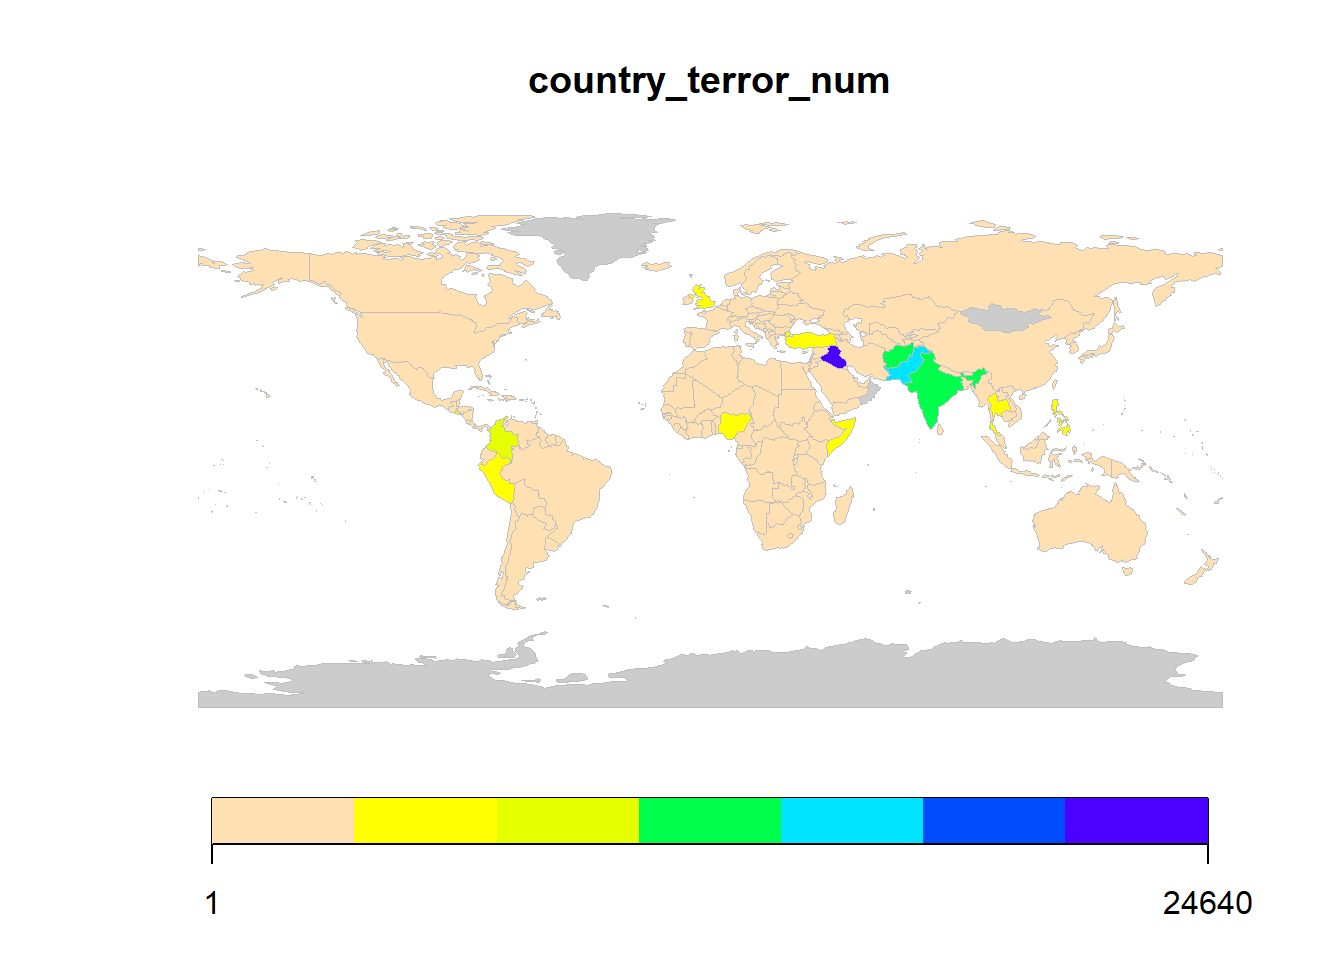
\includegraphics{SSAMethodCode_files/figure-latex/unnamed-chunk-12-1.pdf}

\begin{Shaded}
\begin{Highlighting}[]
\FunctionTok{plot}\NormalTok{(s.TSExample, }\AttributeTok{type=}\StringTok{\textquotesingle{}vectors\textquotesingle{}}\NormalTok{, }\AttributeTok{vectors=}\StringTok{\textquotesingle{}factor\textquotesingle{}}\NormalTok{, }\AttributeTok{idx=}\DecValTok{1}\SpecialCharTok{:}\DecValTok{3}\NormalTok{)}
\end{Highlighting}
\end{Shaded}

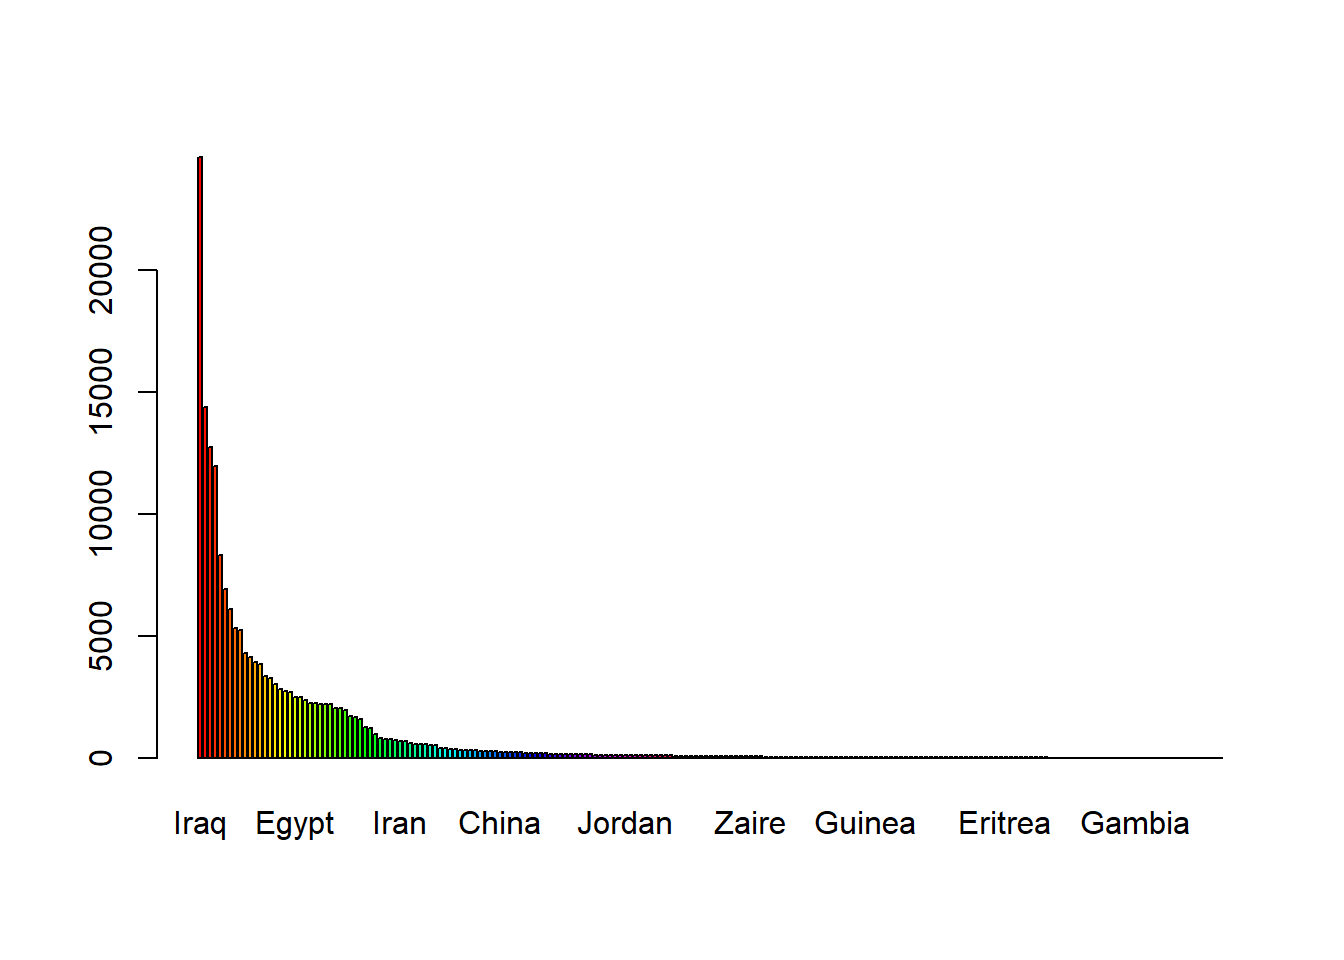
\includegraphics{SSAMethodCode_files/figure-latex/unnamed-chunk-12-2.pdf}

\begin{Shaded}
\begin{Highlighting}[]
\FunctionTok{plot}\NormalTok{(s.TSExample, }\AttributeTok{type=}\StringTok{\textquotesingle{}paired\textquotesingle{}}\NormalTok{, }\AttributeTok{idx=}\DecValTok{1}\SpecialCharTok{:}\DecValTok{2}\NormalTok{, }\AttributeTok{plot.contrib =} \ConstantTok{FALSE}\NormalTok{)}
\end{Highlighting}
\end{Shaded}

\includegraphics{SSAMethodCode_files/figure-latex/unnamed-chunk-12-3.pdf}

\begin{Shaded}
\begin{Highlighting}[]
\FunctionTok{plot}\NormalTok{(s.TSExample, }\AttributeTok{type=}\StringTok{\textquotesingle{}series\textquotesingle{}}\NormalTok{, }\AttributeTok{groups=}\DecValTok{1}\SpecialCharTok{:}\DecValTok{3}\NormalTok{)}
\end{Highlighting}
\end{Shaded}

\includegraphics{SSAMethodCode_files/figure-latex/unnamed-chunk-12-4.pdf}

\begin{Shaded}
\begin{Highlighting}[]
\FunctionTok{plot}\NormalTok{(}\FunctionTok{wcor}\NormalTok{(s.TSExample, }\AttributeTok{groups=}\DecValTok{1}\SpecialCharTok{:}\DecValTok{3}\NormalTok{))}
\end{Highlighting}
\end{Shaded}

\includegraphics{SSAMethodCode_files/figure-latex/unnamed-chunk-12-5.pdf}

\begin{Shaded}
\begin{Highlighting}[]
\FunctionTok{plot}\NormalTok{(r.TSExample)}
\end{Highlighting}
\end{Shaded}

\includegraphics{SSAMethodCode_files/figure-latex/unnamed-chunk-12-6.pdf}

\subsection{Пример 2. Отсутствие
разделимости}\label{ux43fux440ux438ux43cux435ux440-2.-ux43eux442ux441ux443ux442ux441ux442ux432ux438ux435-ux440ux430ux437ux434ux435ux43bux438ux43cux43eux441ux442ux438}

В случае, когда не выполняется слабая разделимость, представление
временной ряд в виде суммы нескольких компонент ряда является
невозможным.

Рассмотрим на простом примере:

Пусть дано два константных ряда. Если мы предполагаем, что они, по
крайней мере, слабо разделимы, то по предложению 2.1, скалярное
произведение произвольных отрезков длины L и K двух рядов должно быть
равно нулю, другими словами, биортогональный базис первого ряда должен
быть ортогонален биортогональному базису второго ряда, поскольку все
элементы ряда образованы некоторым биортогональным базисом сингулярного
значения

\begin{Shaded}
\begin{Highlighting}[]
\NormalTok{ConstTS\_One }\OtherTok{\textless{}{-}} \FunctionTok{rep}\NormalTok{(}\DecValTok{2}\NormalTok{, }\DecValTok{10}\NormalTok{)}

\NormalTok{ConstTS\_Two }\OtherTok{\textless{}{-}} \FunctionTok{rep}\NormalTok{(}\DecValTok{3}\NormalTok{, }\DecValTok{10}\NormalTok{)}

\CommentTok{\# Взяв произвольную длину окна 1 \textless{} L \textless{} 10}

\NormalTok{L }\OtherTok{\textless{}{-}} \DecValTok{6} 
\NormalTok{K }\OtherTok{\textless{}{-}} \DecValTok{10} \SpecialCharTok{{-}}\NormalTok{ L }\SpecialCharTok{+} \DecValTok{1}

\NormalTok{ConstTSValue }\OtherTok{\textless{}{-}} \FunctionTok{c}\NormalTok{(ConstTS\_One[}\DecValTok{2}\SpecialCharTok{:}\NormalTok{(}\DecValTok{1}\SpecialCharTok{+}\NormalTok{L)]}\SpecialCharTok{\%*\%}\NormalTok{ConstTS\_Two[}\DecValTok{4}\SpecialCharTok{:}\NormalTok{(}\DecValTok{3}\SpecialCharTok{+}\NormalTok{L)],}
\NormalTok{ConstTS\_One[}\DecValTok{1}\SpecialCharTok{:}\NormalTok{K]}\SpecialCharTok{\%*\%}\NormalTok{ConstTS\_Two[}\DecValTok{5}\SpecialCharTok{:}\NormalTok{(}\DecValTok{4}\SpecialCharTok{+}\NormalTok{K)])}

\CommentTok{\#видим, что значения скалярное произведение любого отрезка ряда = 6L или}
\CommentTok{\#6K != 0. Следовательно, константные ряды не могут быть отделимы друг от}
\CommentTok{\#друга}

\CommentTok{\# Конец задачи 1.}
\end{Highlighting}
\end{Shaded}

\subsubsection{Замечание: нужно доделать первую задачу через пакет
Rssa.}\label{ux437ux430ux43cux435ux447ux430ux43dux438ux435-ux43dux443ux436ux43dux43e-ux434ux43eux434ux435ux43bux430ux442ux44c-ux43fux435ux440ux432ux443ux44e-ux437ux430ux434ux430ux447ux443-ux447ux435ux440ux435ux437-ux43fux430ux43aux435ux442-rssa.}

\section{Задача 2.}\label{ux437ux430ux434ux430ux447ux430-2.}

На этом шаге обрабатывается таблица значений средних температур по
месяцам. Столбцы - месяцы, строки - года. Чтобы построить временной ряд
из таблицы нужно брать числа слева-направо (то есть, от января до
декабря) и сверху-вниз (от ранних дат до поздних)

\begin{Shaded}
\begin{Highlighting}[]
\NormalTok{spData }\OtherTok{\textless{}{-}} \FunctionTok{read.table}\NormalTok{(}\StringTok{"SPData.txt"}\NormalTok{, }\AttributeTok{skip=}\DecValTok{5}\NormalTok{, }\AttributeTok{col.names=}\FunctionTok{c}\NormalTok{(}\StringTok{"Индекс ВМО"}\NormalTok{, }\StringTok{"Год"}\NormalTok{, }\StringTok{"Январь"}\NormalTok{,}
                                                       \StringTok{"Февраль"}\NormalTok{, }\StringTok{"Март"}\NormalTok{, }\StringTok{"Апрель"}\NormalTok{,}
                                                       \StringTok{"Май"}\NormalTok{, }\StringTok{"Июнь"}\NormalTok{, }\StringTok{"Июль"}\NormalTok{, }\StringTok{"Август"}\NormalTok{,}
                                                       \StringTok{"Сентябрь"}\NormalTok{, }\StringTok{"Октябрь"}\NormalTok{, }\StringTok{"Ноябрь"}\NormalTok{,}
                                                       \StringTok{"Декабрь"}\NormalTok{)) }


\NormalTok{spDataVector }\OtherTok{\textless{}{-}} \FunctionTok{scan}\NormalTok{(}\StringTok{"SPData.txt"}\NormalTok{, }\AttributeTok{skip =} \DecValTok{5}\NormalTok{)}
\NormalTok{spDataVector }\OtherTok{\textless{}{-}}\NormalTok{ spDataVector[}\SpecialCharTok{!}\NormalTok{spDataVector }\SpecialCharTok{\%in\%} \FunctionTok{c}\NormalTok{(}\DecValTok{26063}\NormalTok{, }\DecValTok{1805}\SpecialCharTok{:}\DecValTok{2021}\NormalTok{)]}
\NormalTok{mspSSA }\OtherTok{\textless{}{-}} \FunctionTok{ssa}\NormalTok{(spDataVector, }\AttributeTok{L =} \DecValTok{1296}\NormalTok{)}
\end{Highlighting}
\end{Shaded}

mspSSA

\begin{Shaded}
\begin{Highlighting}[]
\FunctionTok{plot}\NormalTok{(mspSSA)}
\end{Highlighting}
\end{Shaded}

\includegraphics{SSAMethodCode_files/figure-latex/unnamed-chunk-15-1.pdf}

\begin{Shaded}
\begin{Highlighting}[]
\FunctionTok{summary}\NormalTok{(mspSSA)}
\end{Highlighting}
\end{Shaded}

\begin{verbatim}
## 
## Call:
## ssa(x = spDataVector, L = 1296)
## 
## Series length: 2604, Window length: 1296,    SVD method: nutrlan
## Special triples:  0
## 
## Computed:
## Eigenvalues: 50, Eigenvectors: 50,   Factor vectors: 0
## 
## Precached: 0 elementary series (0 MiB)
## 
## Overall memory consumption (estimate): 0.5172 MiB
\end{verbatim}

\begin{Shaded}
\begin{Highlighting}[]
\FunctionTok{plot}\NormalTok{(mspSSA, }\AttributeTok{type=}\StringTok{\textquotesingle{}vectors\textquotesingle{}}\NormalTok{, }\AttributeTok{idx=}\DecValTok{1}\SpecialCharTok{:}\DecValTok{16}\NormalTok{)}
\end{Highlighting}
\end{Shaded}

\includegraphics{SSAMethodCode_files/figure-latex/unnamed-chunk-15-2.pdf}

\begin{Shaded}
\begin{Highlighting}[]
\FunctionTok{plot}\NormalTok{(mspSSA, }\AttributeTok{type=}\StringTok{\textquotesingle{}vectors\textquotesingle{}}\NormalTok{, }\AttributeTok{vectors=}\StringTok{\textquotesingle{}factor\textquotesingle{}}\NormalTok{, }\AttributeTok{idx=}\DecValTok{1}\SpecialCharTok{:}\DecValTok{16}\NormalTok{)}
\end{Highlighting}
\end{Shaded}

\includegraphics{SSAMethodCode_files/figure-latex/unnamed-chunk-15-3.pdf}

\begin{Shaded}
\begin{Highlighting}[]
\FunctionTok{plot}\NormalTok{(mspSSA, }\AttributeTok{type=}\StringTok{\textquotesingle{}series\textquotesingle{}}\NormalTok{, }\AttributeTok{groups=}\DecValTok{1}\SpecialCharTok{:}\DecValTok{16}\NormalTok{)}
\end{Highlighting}
\end{Shaded}

\includegraphics{SSAMethodCode_files/figure-latex/unnamed-chunk-15-4.pdf}

Поскольку длина окна близка к числу окон, то графики их собственных и
факторных векторов совпадают. Первые две компоненты вносят наибольший
вклад и, исходя из близости собственных чисел, являются колебаниями.
Тоже самое можно сказать и про пары, идущие после 3-ей собственной
тройки.

\begin{Shaded}
\begin{Highlighting}[]
\FunctionTok{plot}\NormalTok{(mspSSA, }\AttributeTok{type=}\StringTok{"paired"}\NormalTok{, }\AttributeTok{idx=}\DecValTok{1}\SpecialCharTok{:}\DecValTok{12}\NormalTok{, }\AttributeTok{plot.contrib =} \ConstantTok{FALSE}\NormalTok{)}
\end{Highlighting}
\end{Shaded}

\includegraphics{SSAMethodCode_files/figure-latex/unnamed-chunk-16-1.pdf}

\begin{Shaded}
\begin{Highlighting}[]
\FunctionTok{plot}\NormalTok{(}\FunctionTok{wcor}\NormalTok{(mspSSA, }\AttributeTok{groups=}\DecValTok{1}\SpecialCharTok{:}\DecValTok{31}\NormalTok{), }\AttributeTok{scales=}\FunctionTok{list}\NormalTok{(}\AttributeTok{at=}\FunctionTok{seq}\NormalTok{(}\DecValTok{5}\NormalTok{,}\DecValTok{30}\NormalTok{,}\DecValTok{5}\NormalTok{)))}
\end{Highlighting}
\end{Shaded}

\includegraphics{SSAMethodCode_files/figure-latex/unnamed-chunk-16-2.pdf}

Анализируя пары собственных векторов, можно заметить что у первой пары
явно выраженный период, равный 1/12. В то же время, период второй пары
собственных векторов, 4-ой и 5-ой, равен 1/6. Таким образом, основное
воздействие на температуру в Санкт-Петербурге оказывали сезонные
изменения, происходившие ежемесячно. Так, можно предположить, что этими
изменениями была переменчивая погода города.

Если говорить про единственный тренд, являющийся 3-ей собственной
тройкой, то можно интерпретировать его как сохраняющий уровень
температуры фактор, например, воздействие солнца.

\subsubsection{Восстановление утраченных
действий}\label{ux432ux43eux441ux441ux442ux430ux43dux43eux432ux43bux435ux43dux438ux435-ux443ux442ux440ux430ux447ux435ux43dux43dux44bux445-ux434ux435ux439ux441ux442ux432ux438ux439}

\begin{Shaded}
\begin{Highlighting}[]
\NormalTok{s.mspSSA }\OtherTok{\textless{}{-}} \FunctionTok{ssa}\NormalTok{(spDataVector , }\AttributeTok{L=}\DecValTok{1296}\NormalTok{, }\AttributeTok{neig=}\DecValTok{300}\NormalTok{)}
\NormalTok{g.mspSSA }\OtherTok{\textless{}{-}} \FunctionTok{grouping.auto}\NormalTok{(s.mspSSA, }\AttributeTok{base=}\StringTok{\textquotesingle{}series\textquotesingle{}}\NormalTok{, }\AttributeTok{freq.bins=}\FunctionTok{c}\NormalTok{(}\FloatTok{0.1}\NormalTok{,}\FloatTok{0.2}\NormalTok{,}\FloatTok{0.3}\NormalTok{,}\FloatTok{0.4}\NormalTok{,}\SpecialCharTok{+}\ConstantTok{Inf}\NormalTok{))}
\NormalTok{r.mspSSA }\OtherTok{\textless{}{-}} \FunctionTok{reconstruct}\NormalTok{(s.mspSSA, }\AttributeTok{groups=}\FunctionTok{list}\NormalTok{(}\AttributeTok{Trend =} \DecValTok{3}\NormalTok{, }\AttributeTok{Seasonality=}\FunctionTok{c}\NormalTok{(}\DecValTok{1}\SpecialCharTok{:}\DecValTok{2}\NormalTok{,}\DecValTok{4}\SpecialCharTok{:}\DecValTok{5}\NormalTok{,}\DecValTok{30}\SpecialCharTok{:}\DecValTok{31}\NormalTok{)))}
\end{Highlighting}
\end{Shaded}

\begin{Shaded}
\begin{Highlighting}[]
\FunctionTok{plot}\NormalTok{(mspSSA, }\AttributeTok{type=}\StringTok{\textquotesingle{}paired\textquotesingle{}}\NormalTok{, }\AttributeTok{idx=}\FunctionTok{c}\NormalTok{(}\DecValTok{1}\NormalTok{,}\DecValTok{4}\NormalTok{,}\DecValTok{30}\NormalTok{), }\AttributeTok{plot.contrib =} \ConstantTok{FALSE}\NormalTok{)}
\end{Highlighting}
\end{Shaded}

\includegraphics{SSAMethodCode_files/figure-latex/unnamed-chunk-18-1.pdf}

\begin{Shaded}
\begin{Highlighting}[]
\FunctionTok{plot}\NormalTok{(}\FunctionTok{reconstruct}\NormalTok{(s.mspSSA, }\AttributeTok{groups=}\FunctionTok{list}\NormalTok{(}\AttributeTok{G12=}\DecValTok{1}\SpecialCharTok{:}\DecValTok{2}\NormalTok{, }\AttributeTok{G6=}\DecValTok{4}\SpecialCharTok{:}\DecValTok{5}\NormalTok{, }\AttributeTok{G4=}\DecValTok{30}\SpecialCharTok{:}\DecValTok{31}\NormalTok{)), }\AttributeTok{plot.method=}\StringTok{"xyplot"}\NormalTok{, }\AttributeTok{layout=}\FunctionTok{c}\NormalTok{(}\DecValTok{2}\NormalTok{,}\DecValTok{2}\NormalTok{))}
\end{Highlighting}
\end{Shaded}

\includegraphics{SSAMethodCode_files/figure-latex/unnamed-chunk-18-2.pdf}
\includegraphics{SSAMethodCode_files/figure-latex/unnamed-chunk-18-3.pdf}

\begin{Shaded}
\begin{Highlighting}[]
\FunctionTok{plot}\NormalTok{(mspSSA, }\AttributeTok{type=}\StringTok{\textquotesingle{}paired\textquotesingle{}}\NormalTok{, }\AttributeTok{vectors=}\StringTok{"factor"}\NormalTok{, }\AttributeTok{idx=}\FunctionTok{c}\NormalTok{(}\DecValTok{1}\NormalTok{,}\DecValTok{4}\NormalTok{,}\DecValTok{30}\NormalTok{), }\AttributeTok{plot.contrib =} \ConstantTok{FALSE}\NormalTok{)}
\end{Highlighting}
\end{Shaded}

\includegraphics{SSAMethodCode_files/figure-latex/unnamed-chunk-18-4.pdf}

\begin{Shaded}
\begin{Highlighting}[]
\FunctionTok{plot}\NormalTok{(}\FunctionTok{wcor}\NormalTok{(mspSSA,}\AttributeTok{groups=}\DecValTok{1}\SpecialCharTok{:}\DecValTok{31}\NormalTok{), }\AttributeTok{scales=}\FunctionTok{list}\NormalTok{(}\AttributeTok{at=}\FunctionTok{seq}\NormalTok{(}\DecValTok{5}\NormalTok{,}\DecValTok{30}\NormalTok{,}\DecValTok{5}\NormalTok{)))}
\end{Highlighting}
\end{Shaded}

\includegraphics{SSAMethodCode_files/figure-latex/unnamed-chunk-18-5.pdf}

\begin{Shaded}
\begin{Highlighting}[]
\FunctionTok{plot}\NormalTok{(}\FunctionTok{wcor}\NormalTok{(mspSSA,}\AttributeTok{groups=}\DecValTok{32}\SpecialCharTok{:}\DecValTok{60}\NormalTok{), }\AttributeTok{scales=}\FunctionTok{list}\NormalTok{(}\AttributeTok{at=}\FunctionTok{seq}\NormalTok{(}\DecValTok{5}\NormalTok{,}\DecValTok{25}\NormalTok{,}\DecValTok{5}\NormalTok{)))}
\end{Highlighting}
\end{Shaded}

\includegraphics{SSAMethodCode_files/figure-latex/unnamed-chunk-18-6.pdf}

\begin{Shaded}
\begin{Highlighting}[]
\FunctionTok{plot}\NormalTok{(}\FunctionTok{wcor}\NormalTok{(mspSSA, }\AttributeTok{groups=}\DecValTok{1}\SpecialCharTok{:}\DecValTok{60}\NormalTok{), }\AttributeTok{scales=}\FunctionTok{list}\NormalTok{(}\AttributeTok{at=}\FunctionTok{seq}\NormalTok{(}\DecValTok{5}\NormalTok{,}\DecValTok{60}\NormalTok{,}\DecValTok{5}\NormalTok{)))}
\end{Highlighting}
\end{Shaded}

\includegraphics{SSAMethodCode_files/figure-latex/unnamed-chunk-18-7.pdf}

\begin{Shaded}
\begin{Highlighting}[]
\NormalTok{timecut }\OtherTok{\textless{}{-}} \FunctionTok{window}\NormalTok{(spDataVector, }\AttributeTok{end=}\FunctionTok{time}\NormalTok{(spDataVector)[}\DecValTok{169}\NormalTok{])}
\end{Highlighting}
\end{Shaded}

\begin{Shaded}
\begin{Highlighting}[]
\NormalTok{r.spTimecut }\OtherTok{\textless{}{-}} \FunctionTok{reconstruct}\NormalTok{(s.mspSSA, }\AttributeTok{groups=}\FunctionTok{list}\NormalTok{(}\AttributeTok{Trend=}\DecValTok{3}\NormalTok{, }\AttributeTok{Seasonality=}\FunctionTok{c}\NormalTok{(}\DecValTok{1}\SpecialCharTok{:}\DecValTok{2}\NormalTok{,}\DecValTok{4}\SpecialCharTok{:}\DecValTok{5}\NormalTok{,}\DecValTok{30}\SpecialCharTok{:}\DecValTok{31}\NormalTok{)))}
\NormalTok{r.spTimecut}\SpecialCharTok{$}\NormalTok{Trend }\OtherTok{\textless{}{-}}\NormalTok{ r.spTimecut}\SpecialCharTok{$}\NormalTok{Trend[}\DecValTok{1}\SpecialCharTok{:}\DecValTok{241}\NormalTok{]}
\NormalTok{r.spTimecut}\SpecialCharTok{$}\NormalTok{Seasonality }\OtherTok{\textless{}{-}}\NormalTok{ r.spTimecut}\SpecialCharTok{$}\NormalTok{Seasonality[}\DecValTok{1}\SpecialCharTok{:}\DecValTok{241}\NormalTok{]}

\NormalTok{r.spTimecutSeason }\OtherTok{\textless{}{-}} \FunctionTok{reconstruct}\NormalTok{(s.mspSSA, }\AttributeTok{groups=}\FunctionTok{list}\NormalTok{(}\AttributeTok{G12=}\DecValTok{1}\SpecialCharTok{:}\DecValTok{2}\NormalTok{, }\AttributeTok{G6=}\DecValTok{4}\SpecialCharTok{:}\DecValTok{5}\NormalTok{, }\AttributeTok{G4=}\DecValTok{30}\SpecialCharTok{:}\DecValTok{31}\NormalTok{))}
\NormalTok{r.spTimecutSeason}\SpecialCharTok{$}\NormalTok{G12 }\OtherTok{\textless{}{-}}\NormalTok{ r.spTimecutSeason}\SpecialCharTok{$}\NormalTok{G12[}\DecValTok{1}\SpecialCharTok{:}\DecValTok{241}\NormalTok{]}
\NormalTok{r.spTimecutSeason}\SpecialCharTok{$}\NormalTok{G6 }\OtherTok{\textless{}{-}}\NormalTok{ r.spTimecutSeason}\SpecialCharTok{$}\NormalTok{G6[}\DecValTok{1}\SpecialCharTok{:}\DecValTok{241}\NormalTok{]}
\NormalTok{r.spTimecutSeason}\SpecialCharTok{$}\NormalTok{G4 }\OtherTok{\textless{}{-}}\NormalTok{ r.spTimecutSeason}\SpecialCharTok{$}\NormalTok{G4[}\DecValTok{1}\SpecialCharTok{:}\DecValTok{241}\NormalTok{]}
\end{Highlighting}
\end{Shaded}

\begin{Shaded}
\begin{Highlighting}[]
\FunctionTok{plot}\NormalTok{(r.spTimecut, }\AttributeTok{add.residuals=}\ConstantTok{TRUE}\NormalTok{, }\AttributeTok{add.original=}\ConstantTok{TRUE}\NormalTok{, }\AttributeTok{plot.method=}\StringTok{\textquotesingle{}xyplot\textquotesingle{}}\NormalTok{, }\AttributeTok{superpose=}\ConstantTok{TRUE}\NormalTok{, }\AttributeTok{layout=}\FunctionTok{c}\NormalTok{(}\DecValTok{2}\NormalTok{,}\DecValTok{2}\NormalTok{))}
\end{Highlighting}
\end{Shaded}

\begin{verbatim}
## Warning in cbind(original, m): number of rows of result is not a multiple of
## vector length (arg 1)
\end{verbatim}

\begin{verbatim}
## Warning in cbind(m, res): number of rows of result is not a multiple of vector
## length (arg 2)
\end{verbatim}

\includegraphics{SSAMethodCode_files/figure-latex/unnamed-chunk-21-1.pdf}

\begin{Shaded}
\begin{Highlighting}[]
\FunctionTok{plot}\NormalTok{(r.spTimecutSeason, }\AttributeTok{add.residuals=}\ConstantTok{FALSE}\NormalTok{, }\AttributeTok{add.original=}\ConstantTok{FALSE}\NormalTok{, }\AttributeTok{plot.method=}\StringTok{\textquotesingle{}xyplot\textquotesingle{}}\NormalTok{, }\AttributeTok{superpose=}\ConstantTok{TRUE}\NormalTok{, }\AttributeTok{layout=}\FunctionTok{c}\NormalTok{(}\DecValTok{2}\NormalTok{,}\DecValTok{2}\NormalTok{))}
\end{Highlighting}
\end{Shaded}

\includegraphics{SSAMethodCode_files/figure-latex/unnamed-chunk-21-2.pdf}

\subsection{Замечания}\label{ux437ux430ux43cux435ux447ux430ux43dux438ux44f}

Денис, здравствуйте!

Сделано хорошо, видно, что разобрались.

Возникло несколько вопросов.

\begin{enumerate}
\def\labelenumi{\arabic{enumi}.}
\tightlist
\item
  Первое ---~как каждый из графиков 1-3 показывает (подтверждает), что
  есть сильная разделимость? (у вас нет комментариев) +
\item
  Примером отсутствия слабой разделимости может, вероятно, служить
  случай другой частоты, не 1/4? Две константы ---~вырожденный пример.

  \begin{itemize}
  \tightlist
  \item
  \end{itemize}
\item
  Про шум не поняла. Шум ---~случайная составляющая, для него
  теоретически вы не можете получить результат, но можете
  продемонстрировать, что при увеличении N точность выделения компонент
  возрастает. +
\item
  В реальном примере: такой график плохо
  выглядит?~~\url{https://ssa-with-r-book.github.io/01-chapter2-part1.html\#produced-output}

  \begin{itemize}
  \tightlist
  \item
  \end{itemize}
\end{enumerate}

\subsection{Новые
изменения}\label{ux43dux43eux432ux44bux435-ux438ux437ux43cux435ux43dux435ux43dux438ux44f}

\begin{Shaded}
\begin{Highlighting}[]
\FunctionTok{library}\NormalTok{(}\StringTok{"Rssa"}\NormalTok{)}
\FunctionTok{data}\NormalTok{(}\StringTok{"AustralianWine"}\NormalTok{, }\AttributeTok{package =} \StringTok{"Rssa"}\NormalTok{)}
\NormalTok{fort }\OtherTok{\textless{}{-}} \FunctionTok{window}\NormalTok{(AustralianWine, }\AttributeTok{end =} \FunctionTok{time}\NormalTok{(AustralianWine)[}\DecValTok{174}\NormalTok{])}
\NormalTok{fort}\OtherTok{\textless{}{-}}\NormalTok{fort[,}\StringTok{"Fortified"}\NormalTok{]}
\end{Highlighting}
\end{Shaded}

\begin{Shaded}
\begin{Highlighting}[]
\NormalTok{s.fort }\OtherTok{\textless{}{-}} \FunctionTok{ssa}\NormalTok{(fort, }\AttributeTok{L =} \DecValTok{84}\NormalTok{, }\AttributeTok{kind =} \StringTok{"1d{-}ssa"}\NormalTok{)}
\NormalTok{r.fort }\OtherTok{\textless{}{-}} \FunctionTok{reconstruct}\NormalTok{(s.fort, }
                      \AttributeTok{groups =} \FunctionTok{list}\NormalTok{(}\AttributeTok{Trend =} \DecValTok{1}\NormalTok{,}
                                    \AttributeTok{Seasonality =} \DecValTok{2}\SpecialCharTok{:}\DecValTok{11}\NormalTok{))}
\FunctionTok{plot}\NormalTok{(r.fort, }\AttributeTok{add.residuals =} \ConstantTok{TRUE}\NormalTok{, }\AttributeTok{add.original =} \ConstantTok{TRUE}\NormalTok{,}
     \AttributeTok{plot.method =} \StringTok{"xyplot"}\NormalTok{,}
     \AttributeTok{superpose =} \ConstantTok{TRUE}\NormalTok{, }\AttributeTok{auto.key =} \FunctionTok{list}\NormalTok{(}\AttributeTok{columns =} \DecValTok{2}\NormalTok{))}
\end{Highlighting}
\end{Shaded}

\includegraphics{SSAMethodCode_files/figure-latex/unnamed-chunk-23-1.pdf}

\begin{Shaded}
\begin{Highlighting}[]
\NormalTok{s.mspSSA }\OtherTok{\textless{}{-}} \FunctionTok{ssa}\NormalTok{(spDataVector , }\AttributeTok{L=}\DecValTok{1296}\NormalTok{, }\AttributeTok{neig=}\DecValTok{300}\NormalTok{)}
\NormalTok{r.mspSSA }\OtherTok{\textless{}{-}} \FunctionTok{reconstruct}\NormalTok{(s.mspSSA, }\AttributeTok{groups=}\FunctionTok{list}\NormalTok{(}\AttributeTok{Trend =} \DecValTok{3}\NormalTok{, }\AttributeTok{Seasonality=}\FunctionTok{c}\NormalTok{(}\DecValTok{1}\SpecialCharTok{:}\DecValTok{2}\NormalTok{,}\DecValTok{4}\SpecialCharTok{:}\DecValTok{5}\NormalTok{,}\DecValTok{30}\SpecialCharTok{:}\DecValTok{31}\NormalTok{)))}
\FunctionTok{par}\NormalTok{(}\AttributeTok{mar=}\FunctionTok{c}\NormalTok{(}\DecValTok{3}\NormalTok{,}\DecValTok{2}\NormalTok{,}\DecValTok{5}\NormalTok{,}\DecValTok{1}\NormalTok{), }\AttributeTok{xpd=}\ConstantTok{FALSE}\NormalTok{)}

\FunctionTok{plot}\NormalTok{(r.mspSSA, }\AttributeTok{add.residuals=}\ConstantTok{TRUE}\NormalTok{, }\AttributeTok{add.original=}\ConstantTok{FALSE}\NormalTok{, }\AttributeTok{col=}\FunctionTok{c}\NormalTok{(}\StringTok{\textquotesingle{}white\textquotesingle{}}\NormalTok{, }\StringTok{\textquotesingle{}green\textquotesingle{}}\NormalTok{, }\StringTok{\textquotesingle{}purple\textquotesingle{}}\NormalTok{), }\AttributeTok{lty=}\FunctionTok{c}\NormalTok{(}\DecValTok{0}\NormalTok{, }\DecValTok{1}\NormalTok{, }\DecValTok{1}\NormalTok{), }\AttributeTok{xlim=}\FunctionTok{c}\NormalTok{(}\DecValTok{0}\NormalTok{,}\DecValTok{250}\NormalTok{))}

\FunctionTok{legend}\NormalTok{(}\StringTok{\textquotesingle{}bottomright\textquotesingle{}}\NormalTok{, }\AttributeTok{legend=}\FunctionTok{c}\NormalTok{(}\StringTok{\textquotesingle{}Seasonality\textquotesingle{}}\NormalTok{, }\StringTok{\textquotesingle{}Residuals\textquotesingle{}}\NormalTok{), }\AttributeTok{pch=}\FunctionTok{rep}\NormalTok{(}\DecValTok{15}\NormalTok{,}\DecValTok{4}\NormalTok{), }\AttributeTok{col=}\FunctionTok{c}\NormalTok{(}\StringTok{\textquotesingle{}green\textquotesingle{}}\NormalTok{,}\StringTok{\textquotesingle{}purple\textquotesingle{}}\NormalTok{), }\AttributeTok{cex=}\FloatTok{0.7}\NormalTok{)}
\end{Highlighting}
\end{Shaded}

\includegraphics{SSAMethodCode_files/figure-latex/unnamed-chunk-24-1.pdf}

\begin{Shaded}
\begin{Highlighting}[]
\FunctionTok{plot}\NormalTok{(r.mspSSA, }\AttributeTok{add.residuals=}\ConstantTok{TRUE}\NormalTok{, }\AttributeTok{add.original=}\ConstantTok{FALSE}\NormalTok{, }\AttributeTok{col=}\FunctionTok{c}\NormalTok{(}\StringTok{\textquotesingle{}white\textquotesingle{}}\NormalTok{, }\StringTok{\textquotesingle{}green\textquotesingle{}}\NormalTok{, }\StringTok{\textquotesingle{}purple\textquotesingle{}}\NormalTok{), }\AttributeTok{lty=}\FunctionTok{c}\NormalTok{(}\DecValTok{0}\NormalTok{, }\DecValTok{0}\NormalTok{, }\DecValTok{1}\NormalTok{))}

\FunctionTok{legend}\NormalTok{(}\StringTok{\textquotesingle{}bottomright\textquotesingle{}}\NormalTok{, }\AttributeTok{legend=}\FunctionTok{c}\NormalTok{(}\StringTok{\textquotesingle{}Residuals\textquotesingle{}}\NormalTok{), }\AttributeTok{pch=}\FunctionTok{rep}\NormalTok{(}\DecValTok{15}\NormalTok{,}\DecValTok{4}\NormalTok{), }\AttributeTok{col=}\FunctionTok{c}\NormalTok{(}\StringTok{\textquotesingle{}purple\textquotesingle{}}\NormalTok{), }\AttributeTok{cex=}\FloatTok{0.7}\NormalTok{)}
\end{Highlighting}
\end{Shaded}

\includegraphics{SSAMethodCode_files/figure-latex/unnamed-chunk-25-1.pdf}

\begin{Shaded}
\begin{Highlighting}[]
\FunctionTok{plot}\NormalTok{(r.mspSSA, }\AttributeTok{add.residuals=}\ConstantTok{TRUE}\NormalTok{, }\AttributeTok{add.original=}\ConstantTok{FALSE}\NormalTok{, }\AttributeTok{col=}\FunctionTok{c}\NormalTok{(}\StringTok{\textquotesingle{}red\textquotesingle{}}\NormalTok{, }\StringTok{\textquotesingle{}green\textquotesingle{}}\NormalTok{, }\StringTok{\textquotesingle{}purple\textquotesingle{}}\NormalTok{), }\AttributeTok{lty=}\FunctionTok{c}\NormalTok{(}\DecValTok{0}\NormalTok{, }\DecValTok{1}\NormalTok{, }\DecValTok{1}\NormalTok{))}

\FunctionTok{legend}\NormalTok{(}\StringTok{\textquotesingle{}bottomright\textquotesingle{}}\NormalTok{, }\AttributeTok{legend=}\FunctionTok{c}\NormalTok{(}\StringTok{\textquotesingle{}Seasonality\textquotesingle{}}\NormalTok{, }\StringTok{\textquotesingle{}Residuals\textquotesingle{}}\NormalTok{), }\AttributeTok{pch=}\FunctionTok{rep}\NormalTok{(}\DecValTok{15}\NormalTok{,}\DecValTok{2}\NormalTok{), }\AttributeTok{col=}\FunctionTok{c}\NormalTok{(}\StringTok{\textquotesingle{}green\textquotesingle{}}\NormalTok{,}\StringTok{\textquotesingle{}purple\textquotesingle{}}\NormalTok{), }\AttributeTok{cex=}\FloatTok{0.7}\NormalTok{)}
\end{Highlighting}
\end{Shaded}

\includegraphics{SSAMethodCode_files/figure-latex/unnamed-chunk-26-1.pdf}

\begin{Shaded}
\begin{Highlighting}[]
\FunctionTok{plot}\NormalTok{(r.mspSSA, }\AttributeTok{add.residuals=}\ConstantTok{FALSE}\NormalTok{, }\AttributeTok{add.original=}\ConstantTok{TRUE}\NormalTok{, }\AttributeTok{col=}\FunctionTok{c}\NormalTok{(}\StringTok{\textquotesingle{}black\textquotesingle{}}\NormalTok{, }\StringTok{\textquotesingle{}red\textquotesingle{}}\NormalTok{, }\StringTok{\textquotesingle{}purple\textquotesingle{}}\NormalTok{), }\AttributeTok{lty=}\FunctionTok{c}\NormalTok{(}\DecValTok{1}\NormalTok{, }\DecValTok{1}\NormalTok{, }\DecValTok{0}\NormalTok{))}

\FunctionTok{legend}\NormalTok{(}\StringTok{\textquotesingle{}bottomright\textquotesingle{}}\NormalTok{, }\AttributeTok{legend=}\FunctionTok{c}\NormalTok{(}\StringTok{\textquotesingle{}Original\textquotesingle{}}\NormalTok{, }\StringTok{\textquotesingle{}Trend\textquotesingle{}}\NormalTok{), }\AttributeTok{pch=}\FunctionTok{rep}\NormalTok{(}\DecValTok{15}\NormalTok{,}\DecValTok{3}\NormalTok{), }\AttributeTok{col=}\FunctionTok{c}\NormalTok{(}\StringTok{\textquotesingle{}black\textquotesingle{}}\NormalTok{,}\StringTok{\textquotesingle{}red\textquotesingle{}}\NormalTok{), }\AttributeTok{cex=}\FloatTok{0.7}\NormalTok{)}
\end{Highlighting}
\end{Shaded}

\includegraphics{SSAMethodCode_files/figure-latex/unnamed-chunk-27-1.pdf}

\section{Новые замечания
(2)}\label{ux43dux43eux432ux44bux435-ux437ux430ux43cux435ux447ux430ux43dux438ux44f-2}

Денис, здравствуйте!

Уточню:~

\begin{enumerate}
\def\labelenumi{\arabic{enumi}.}
\item
  в вашем дополнении в 2.1.2 при чем тут \textbackslash omega
  \textbackslash neq 1/N?~ (а почему там звездочки, а не просто номера
  формул ---~там же, если добавить новые номера, старые автоматически
  меняются?) +
\item
  я все же не поняла, а что вы понимаете под словом «шум», что значит,
  что пример с шумом, где он в описании? +
\item
  реальный пример ---~да, глобальное потепление видно. Случайная
  составляющая ---~это все кроме тренда и сезонности. На графике, где
  рисуете сезонность, имеет смысл рисовать случайную составляющую, чтобы
  сопоставить ее масштаб и масштаб сезонности, а также проверить, что
  остаток (случайная составляющая) колеблется вокруг нуля. +
\end{enumerate}

НЭ

\subsection{Исправления:}\label{ux438ux441ux43fux440ux430ux432ux43bux435ux43dux438ux44f}

\end{document}
